% /*
%  * ----------------------------------------------------------------------------
%  * "THE BEER-WARE LICENSE" (Revision 42):
%  * <michi.wieland@hotmail.com> wrote this file. As long as you retain this notice you
%  * can do whatever you want with this stuff. If we meet some day, and you think
%  * this stuff is worth it, you can buy me a beer in return. Michael Wieland
%  * ----------------------------------------------------------------------------
%  */

\documentclass[
a4paper,
oneside,
10pt,
fleqn,
headsepline,
toc=listofnumbered, 
bibliography=totocnumbered]{scrartcl}

% deutsche Trennmuster etc.
\usepackage[T1]{fontenc}
\usepackage[utf8]{inputenc}
\usepackage[english, ngerman]{babel} % \selectlanguage{english} if  needed
\usepackage{lmodern} % use modern latin fonts

% Custom commands
\newcommand{\AUTHOR}{Michael Wieland}
\newcommand{\INSTITUTE}{Hochschule für Technik Rapperswil}
\newcommand{\GITHUB}{https://github.com/michiwieland/hsr-zusammenfassungen}
\newcommand{\LICENSEURL}{https://en.wikipedia.org/wiki/Beerware}
\newcommand{\LICENSE}{
"THE BEER-WARE LICENSE" (Revision 42):
<michi.wieland@hotmail.com> wrote this file. As long as you retain this notice you
can do whatever you want with this stuff. If we meet some day, and you think
this stuff is worth it, you can buy me a beer in return. Michael Wieland	
}

% Jede Überschrift 1 auf neuer Seite
\let\stdsection\section
\renewcommand\section{\clearpage\stdsection}

% Multiple Authors
\usepackage{authblk}

% Include external pdf
\usepackage{pdfpages}

% Layout / Seitenränder
\usepackage{geometry}

% Inhaltsverzeichnis
\usepackage{makeidx} 
\makeindex

\usepackage{url}
\usepackage[pdfborder={0 0 0}]{hyperref}
\usepackage[all]{hypcap}
\usepackage{hyperxmp} % for license metadata

% Glossar und Abkürzungsverzeichnis
\usepackage[acronym,toc,nopostdot]{glossaries}
\glossarystyle{altlist}
\usepackage{xparse}
\DeclareDocumentCommand{\newdualentry}{ O{} O{} m m m m } {
	\newglossaryentry{gls-#3}{
		name={#4 : #5},
		text={#5\glsadd{#3}},
		description={#6},
		#1
	}
	\makeglossaries
	\newacronym[see={[Siehe:]{gls-#3}},#2]{#3}{#4}{#5\glsadd{gls-#3}}
}
\makeglossaries

% Mathematik
\usepackage{amsmath}
\usepackage{amssymb}
\usepackage{amsfonts}
\usepackage{enumitem}

% Images
\usepackage{graphicx}
\graphicspath{{images/}} % default paths

% Boxes
\usepackage{fancybox}

%Tables
\usepackage{tabu}
\usepackage{booktabs} % toprule, midrule, bottomrule
\usepackage{array} % for matrix tables

% Multi Columns
\usepackage{multicol}

% Header and footer
\usepackage{scrlayer-scrpage}
\setkomafont{pagehead}{\normalfont}
\setkomafont{pagefoot}{\normalfont}
\automark*{section}
\clearpairofpagestyles
\ihead{\headmark}
\ohead{\AUTHOR}
\cfoot{\pagemark}

% Pseudocode
\usepackage{algorithmic}
\usepackage[linesnumbered,ruled]{algorithm2e}

% Code Listings
\usepackage{listings}
\usepackage{color}
\usepackage{beramono}

\definecolor{bluekeywords}{rgb}{0,0,1}
\definecolor{greencomments}{rgb}{0,0.5,0}
\definecolor{redstrings}{rgb}{0.64,0.08,0.08}
\definecolor{xmlcomments}{rgb}{0.5,0.5,0.5}
\definecolor{types}{rgb}{0.17,0.57,0.68}

\lstdefinestyle{visual-studio-style}{
	language=[Sharp]C,
	columns=flexible,
	showstringspaces=false,
	basicstyle=\footnotesize\ttfamily, 
	commentstyle=\color{greencomments},
	morekeywords={partial, var, value, get, set},
	keywordstyle=\bfseries\color{bluekeywords},
	stringstyle=\color{redstrings},
	breaklines=true,
	breakatwhitespace=true,
	tabsize=4,
	numbers=left,
	numberstyle=\tiny\color{black},
	frame=lines,
	showspaces=false,
	showtabs=false,
	escapeinside={£}{£},
}

\definecolor{DarkPurple}{rgb}{0.4, 0.1, 0.4}
\definecolor{DarkCyan}{rgb}{0.0, 0.5, 0.4}
\definecolor{LightLime}{rgb}{0.3, 0.5, 0.4}
\definecolor{Blue}{rgb}{0.0, 0.0, 1.0}

\lstdefinestyle{cevelop-style}{
	language=C++,  
	columns=flexible,
	showstringspaces=false,     
	basicstyle=\footnotesize\ttfamily, 
	keywordstyle=\bfseries\color{DarkPurple},
	commentstyle=\color{LightLime},
	stringstyle=\color{Blue}, 
	escapeinside={£}{£}, % latex scope within code      
	breaklines=true,
	breakatwhitespace=true,
	showspaces=false,
	showtabs=false,
	tabsize=4,
	morekeywords={include,ifndef,define},
	numbers=left,
	numberstyle=\tiny\color{black},
	frame=lines,
}

\lstdefinestyle{eclipse-style}{
	language=Java,  
	columns=flexible,
	showstringspaces=false,     
	basicstyle=\footnotesize\ttfamily, 
	keywordstyle=\bfseries\color{DarkPurple},
	commentstyle=\color{LightLime},
	stringstyle=\color{Blue}, 
	escapeinside={£}{£}, % latex scope within code      
	breaklines=true,
	breakatwhitespace=true,
	showspaces=false,
	showtabs=false,
	tabsize=4,
	morekeywords={length},
	numbers=left,
	numberstyle=\tiny\color{black},
	frame=lines,
}
\lstset{style=eclipse-style}



% Theorems \begin{mytheo}{title}{label}
\usepackage{tcolorbox}
\tcbuselibrary{theorems}
\newtcbtheorem[number within=section]{definiton}{Definition}%
{fonttitle=\bfseries}{def}
\newtcbtheorem[number within=section]{remember}{Merke}%
{fonttitle=\bfseries}{rem}
\newtcbtheorem[number within=section]{hint}{Hinweis}%
{fonttitle=\bfseries}{hnt}

% Dokumentinformationen
\newcommand{\SUBJECT}{Zusammenfassung}
\newcommand{\TITLE}{Software Engineering 1}

\loadglsentries{glossar}

% pdf metadata
\hypersetup{
	pdfauthor={\AUTHOR},
	pdftitle={\SUBJECT \TITLE},
	pdfcopyright={\LICENSE},
	pdflicenseurl={\LICENSEURL}
}

\begin{document}
	
% Front page
\title{\TITLE}
\subject{\SUBJECT}
\author{\AUTHOR}
\affil{\INSTITUTE}
\date{\today}
\maketitle

\vfill

% Participate
\paragraph{Mitmachen} \hfill \\
Falls Du an diesem Dokument mitarbeiten willst, kannst Du das Dokument
auf GitHub unter \url{\GITHUB} forken.

% Licence
\paragraph{Lizenz} \hfill \\
\LICENSE

% Table of contents
\tableofcontents


% Glossar and acronyms (if included \loadglsentries{glossar})
\printglossary[type=\acronymtype]
\printglossary
\glsaddall



\section{OOA: Objektorientierte Analyse}
OOA = Statisches Modell + Dynamisches Modell + Contracts

\subsection{Domainanalyse}
Unter Domainanalyse versteht man das Verstehen eines noch unbekannten Problembereichs. Es geht also um eine methodische Analyse des Problems. Des Weiteren betrachtet man das Problem aus einer Black-, und White-Box Sicht. Aus der Domain Analyse resultieren zwei Modelle:
\begin{itemize}
	\item Statisches Modell (Domainmodell)
	\item Dynamisches Modell (Interaktionsdiagramme)
\end{itemize}

\subsection{Probleme im Software Engineering}
Viele Software Projekte laufen nicht zu letzt wegen den folgenden Punkten schief:
\begin{itemize}
	\item Komplexität wird nicht beherrscht
	\item Termine werden überschritten
	\item Kosten werden überschritten
	\item Das Ziel wird verfehlt
	\item Es mangelt an Qualität (evtl. auch auf Grund von fehlender Zeit)
\end{itemize}


\clearpage

\subsection{Statisches Modell}
Das statische Modell ist das \textbf{Domainmodell} mit all seinen Entitäten (Konzepten). Es zerlegt die Problem Domain in verständliche Teile und verzichtet dabei auf Implementierungsdetails wie Fremdschlüssel und Methoden.


\subsubsection{Terminologie}
\paragraph{Domain Modell} \hfill
\begin{itemize}
	\item Das Domain Modell zeigt wesentliche konzeptionelle Klassen und ihre Zusammenhänge, also \textbf{auch Dinge, die nicht persistent werden}.
	\item Im Domain Modell spricht man immer von einem \textbf{Konzept} anstatt von einer Klasse. Der Klassenname wird jedoch oft vom Konzept abgeleitet.
	\item Im Domain Modell sind Assoziationen \textbf{bidirektionale} Beziehungen zwischen Konzepten der realen Welt
	\item Das Domain Modell kann eine Inspiration für das Design Modell sein.
\end{itemize}

\paragraph{Design Modell, Klassenmodell} \hfill
\begin{itemize}
	\item Das Design Modell zeigt persistente Entitäten und ihre Zusammenhänge für eine Realisation.
	\item Das Design Model verfügt \textbf{zusätzlich über Methoden}
	\item Im Design Modell sind Assoziationen \textbf{unidirektionale} Navigationspfade von einem Software Objekt zu einem anderen.
\end{itemize}

\paragraph{Daten Modell} \hfill
\begin{itemize}
	\item Das Daten Modell zeigt persistente Entitäten in der Datenbank (ERD)
\end{itemize}

\subsubsection{Bestandteile}
\paragraph{Nach Larman}
\begin{itemize}
	\item Klassenkonzepte mit Attributen und Beziehungen untereinander, aber ohne Operationen
\end{itemize}

\paragraph{Klassisch}
\begin{itemize}
	\item Klassenkonzepte mit Attributen, Operationen und Beziehungen untereinander
\end{itemize}

\subsubsection{Konzepte}
Konzepte werden im Design Modell zu Klassen. Abstrakte Klassen werden in \textit{Italics} geschrieben

\paragraph{Konzepte ohne Attribute}
Wenn z.B bei Vererbungen bestimmte Childklassen keine Attribute besitzen, muss die Existenzberechtigung der Childklasse überdacht werden.

\paragraph{Vererbung in relationalen DB} \hfill \\
Es gibt zwei Möglichkeiten, eine Vererbungshierarchie in einer relationalen DB abzubilden. Wenn man es mit einem gut entworfenen Vererbungshierarchie zu tun hat, sollte der Table per Hierarchy Ansatz verwendet werden. (die leeren Felder halten sich in Grenzen). Da die Vererbung so oder so relativ viel Schwierigkeiten bereitet, fährt man mit Decoration etc. so oder so besser.
\begin{description}
	\item[Table per Class] Hier wird pro modellierte Klasse eine Tabelle abgelegt. Beim Abruf der Daten für eine abgeleitete Klasse muss ein Join gemacht werden. Dafür gibt es keine Platzverschwendung
	\item[Table per Hierarchy] Hier macht man für die ganze Vererbungs-Hierarchie nur eine Tabelle. Dabei werden nicht benutze Felder leer gelassen.
\end{description}

\paragraph{Aggregation und Komposition} \hfill \\
Aggregation und Komposition sind Teil-Ganzes Beziehungen. Die Diamanten haben in der Regel eine 1-Multiplizität (implizit).
\begin{description}
	\item[Aggregation] Unabhängies Überleben der Teile (weisser Diamant)
	\item[Komposition] Beim Löschen des Ganzen, existieren die Teile auch nicht mehr (schwarzer Diamant)
\end{description}

\begin{figure}[h]
	\centering
	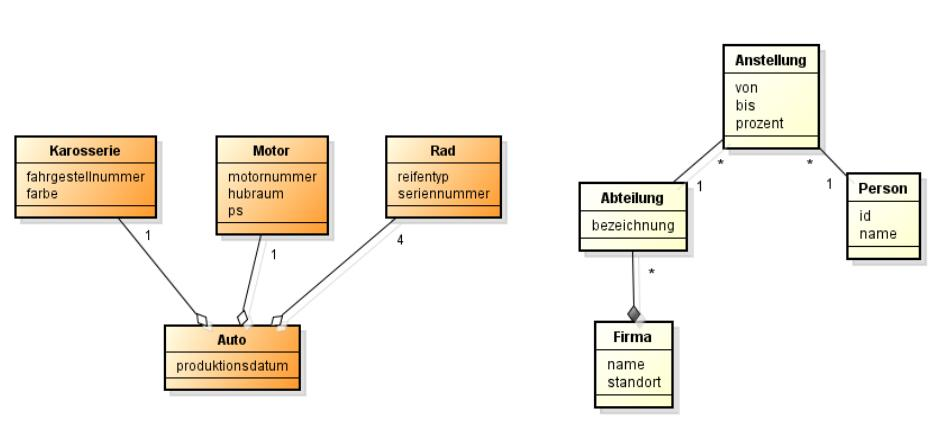
\includegraphics[width=0.7\linewidth]{images/aggregation_komposition}
	\caption{Aggreagation und Komposition}
	\label{fig:aggregationkomposition}
\end{figure}

\subsubsection{Attribute}
Attribute sind logische Datenelemente eines Objekts.

\paragraph{Konzept oder Attribut?}
Ist ein Attribut ein komplexes Objekt, erstellt man für das Attribut besser ein neues Konzept, da man damit flexibler wird. Zum Beispiel würde man das Attribut ''\lstinline|destination|'' des Konzepts ''\lstinline|Flight|'', besser als eigenes Konzept ''\lstinline|Airport|'' mit einem Attribut ''\lstinline|name|'' auslagern.


\paragraph{Auslagern von redundaten Informationen (Beschreibungen)}
Attribute, in welche bei jedem Anlegen der gleiche Wert eingefügt wird, sollten ausgelagert werden. z.B ''\lstinline|description|'' bei dem Konzept ''\lstinline|Kurs|''. In diesem Fall führt man ein neues Konzept ''\lstinline|Kursbeschreibung|'' mit dem Attribut ''\lstinline|description|'' ein. Das neue Konzept ''\lstinline|Kursbeschreibung|'' gilt dann für mehrere ''\lstinline|Kursdurchfuehrungen|''.

\subsubsection{Typen}
Der Typ des Attributs ist im Domain Modell \textbf{optional}. Falls der Typ angegeben wird, muss einer der folgenden verwendet werden.
\begin{itemize}
	\item Boolean
	\item Date
	\item Number
	\item String / Text
	\item Time
\end{itemize}

\subsubsection{Assoziationen}
Eine Assoziation ist eine Beziehung zwischen Konzepten, welche bedeutungsvolle und interessierende Verbindungen (zwischen ihren Instanzen) darstellen. Assoziationen werden immer in die Richtung des Pfeiles gelesen.

\paragraph{1:1 Beziehungen}
\begin{itemize}
	\item 1:1 Beziehungen sind im Domainmodell Ok, im Datenmodell sollten sie jedoch aufgelöst werden
	\item 1:1 Beziehungen machen nur Sinn, wenn die beiden Teile verschiedenen Domänen entstammen oder zu verschiedenen Zeiten erstellt werden.
	\item 1:0..1 Beziehungen sind in beiden Modellen Ok.
\end{itemize}

\paragraph{n:m Beziehungen}
Diese Art von Assoziationen sind zulässig, sehr oft aber nicht richtig, da die Assoziation eigenen Attribute enthält, und deshalb mit einem Zwischenkonzept aufgelöst werden muss. m:n Beziehungen können auf zwei Arten aufgelöst werden:
\begin{enumerate}
	\item Mit Zwischenklasse: Dies ist der Standardfall
	\item Mit Assoziationsklasse: Hier darf jedes Beziehungspaar nur genau einaml vorkommen. (Kombination der zwei Foreign Keys muss unique sein)
\end{enumerate}

\begin{figure}[ht!]
	\begin{minipage}[t]{0.4\textwidth}
		\centering
		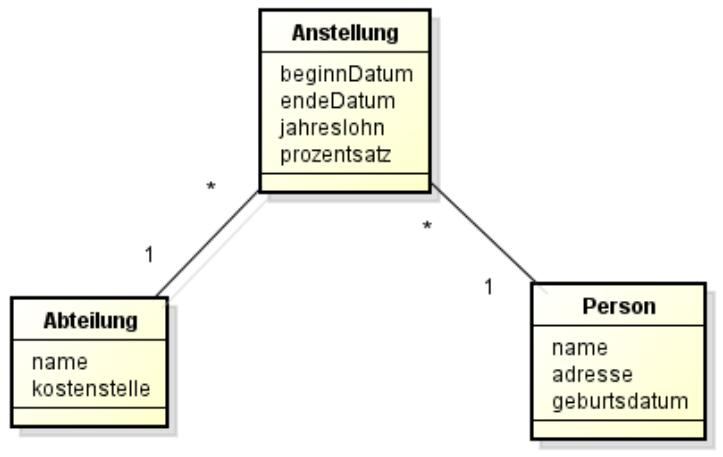
\includegraphics[width=0.7\linewidth]{images/n_m_relation_default}
		\caption{Zwischenklasse für n:m Beziehungen}
		\label{fig:nmrelationdefault}
	\end{minipage}
	\begin{minipage}[t]{0.4\textwidth}
		\centering
		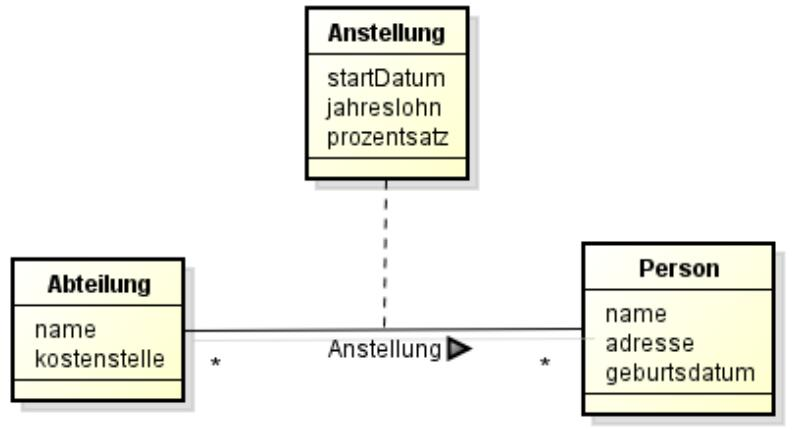
\includegraphics[width=0.7\linewidth]{images/n_m_relation_assoziative}
		\caption{Assoziativklasse für m:n Beziehungen}
		\label{fig:nmrelationassoziative}
	\end{minipage}
\end{figure}


\paragraph{Richtung von Beziehungen in Datenmodell} \hfill \\
Die folgenden Regeln helfen, dass Domainmodelle einfacher zu lesen sind. Sie sind jedoch nur eine Empfehlung.
\begin{enumerate}
	\item Eins-zu-n Beziehungen: eins unten, n darüber
	\item Eins-zu-eins Beziehungen: auf gleicher Höhe
	\item n-zu-m Beziehungen: auf gleicher Höhe
	\item Ableitungen: Basisklasse unten, abgeleitete darüber
\end{enumerate}

\begin{figure}[h]
	\centering
	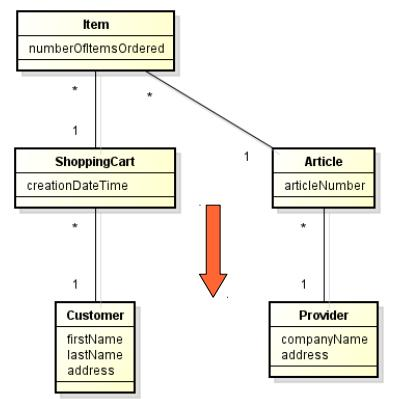
\includegraphics[width=0.5\linewidth]{images/uml_direction}
	\caption{Richtungen von UML Beziehungen}
	\label{fig:umldirection}
\end{figure}

\paragraph{Rollen} \hfill \\
UML bietet die Möglichkeit, eine Beziehung an drei Orten anzuschreiben. Man sollte eine Assoziation immer anschreiben, wenn es mehr als eine Beziehung zwischen zwei Klassen gibt und der Sinn nicht sofort klar ist.
\begin{itemize}
	\item In der Mitte kann man die Art der Beziehung zusammen mit einem Pfeil für die Leserichtung anschreiben.
	\item An jedem Ende der Assoziation kann (je nahe bei einer Klasse) die Rolle, welche die Klasse in der Beziehung spielt, spezifiziert werden.
	\item Ist die Beziehung ein simples (hat ein) dann muss es nicht angeschrieben werden.
\end{itemize}

\clearpage

\subsubsection{Multiplizität}
Die Multiplizität definiert wie viele Instanzen des Types A mit einer Instanz des Types B verbunden sein können.
\begin{table}[h]
	\centering
	\begin{tabu} to \linewidth {l l}
		\toprule
		Multiplizität & Beschreibung \\
		\midrule
		1 & Genau ein \\
		1..* & Ein oder mehrere \\
		* & Keine oder mehrere \\
		n & Genau n \\
		1..n & Ein bis n \\
		x,y,z & x Mal oder y Mal oder z Mal \\
		\bottomrule
	\end{tabu}
	\caption{Multiplizitäten}
\end{table}

\subsubsection{Vorgehen}
\begin{enumerate}
	\item 1x grob durchlesen und Schlüsselwörter notieren
	\item 2-3x genauer durchlesen und Konzepte, Attribute \& Assoziationen identifizieren
	\item Verfeinern: redundantente und falsche Assoziationen löschen
	\item Überprüfen ob alles beachtet wurde
	\item (Evtl. Fragenkatalog und Annahmen bei Unklarheiten)
\end{enumerate}

\subsection{Dynamisches Modell}
Das dynamische Modell bietet eine \textbf{Überprüfung zwischen dem Domain Modell und den effektiven Use Cases}.

\subsubsection{Bestandteile}
\paragraph{Nach Larman}
\begin{itemize}
	\item Black-box Interaktionsdiagramm für Use Case Szenarien
	\item Operation Contracts
	\item Evtl. Zustandsdiagramme für das System oder einzelne Klassen
	\item Aktivitätsdiagramme für einzelne Use Cases
\end{itemize}

\paragraph{Klassisch}
\begin{itemize}
	\item White-box Interaktionsdiagramme für Use Case Szenarien oder Systemoperationen
	\item Evtl: Zustandsdiagramme für System oder einezlne konzeptionelle Klassen
\end{itemize}

\section{Anforderungsanalyse}
In der Anforderungsanalyse oder Requirements Analysis werden die \textbf{Anforderungen an die Software} festgelegt. Man beschreibt was zu realisieren ist (Use Cases) und wer in dem Projekt involviert ist. Es ist empfehlenswert, iterativ vorzugehen, da sich Anforderungen schnell ändern können. Nach der Anforderungsanalyse resultieren folgende Dinge:
\begin{itemize}
	\item Vision
	\item Use Cases und User Stories inkl. Use Case Diagramme
	\item Anforderungsspezifikation (\gls{srs})
	\item Glossar
\end{itemize}


\subsection{SRS: Software Requirements Specification}
\gls{srs} beschreibt verständlich und umfänglich, was die Absicht und die Anforderungen einer Software sind.
\begin{figure}[h]
	\centering
	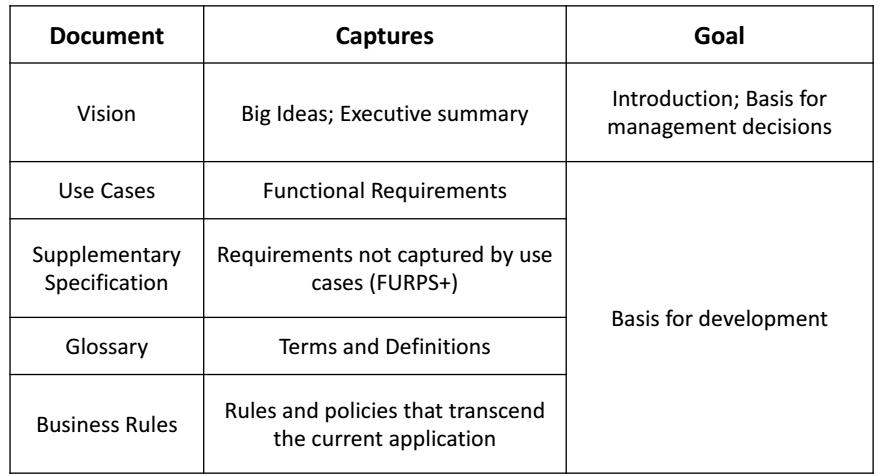
\includegraphics[width=0.7\linewidth]{images/srs_requirements}
	\caption{SRS: Software Requirements Specification}
	\label{fig:srsrequirements}
\end{figure}

\subsection{Klassifikation}
\begin{description}
	\item[Funktionale Anforderungen] \hfill \\
	Funktionale Anfoderungen fragen nach dem Was? Welche Funktionen mit welchen Daten?
	Welche Funktionen, mit welchen Daten
	\item[Nichtfunktionale Anforderungen] \hfill \\
	Nichtfunktionale Anforderungen sind Qualitätsanforderungen und fragen nach dem Wie? Es geht um die Leistung, Menge, Qualitätsmerkmale (Benutzbarkeit, Wartbarkeit), Randbedingungen
	\item[Prozessanforderungen] Kostenschätzung
\end{description}

\subsection{Bestandteile}
\begin{description}
	\item[User Stories] Informale kurze Geschichten aus Benutzersicht (Agile SE)
	\item[Use Cases] Formale Geschichte aus Benutzersicht auf der Ebene elementarer Geschäftsprozesse. 
	\item[Actors] Benutzerrollen in Use Cases
	\item[Personas] Fiktive Personen die den typische Nutzer beschreiben
\end{description}

\subsection{Funktionale Anforderungen}
Funktionale Anforderungen werden mit \textbf{Use Cases} beschreiben. Eine Use Case ist eine textuelle Ablaufbeschreibung mit Ziel und Zweck. (Im Stil: ''Actor macht A, dann macht das System B'') Uses Cases gibt es in drei Formen
\begin{description}
	\item[Brief] \hfill \\
	Kurze Beschreibung (2-3 Sätze; gibt einem eine Idee). Zusammenfassung in einem Abschnitt, beschreibt nur erfolgreiches Szenario
	\item[Casual] \hfill \\
	Mittle Beschreibung (ca. 1/4 Seite). Mehrere Abschnitte, informale Beschreibung mehrerer Szenarien
	\item[Fully dressed] \hfill \\
	Ausführliche Beschreibung. (ca. 2 Seiten) Alle Szenarien im Detail beschrieben, mit Raster für ergänzende Abschnitte, wie Vorbedingungen und Nachbedingungen.
\end{description}


\begin{lstlisting}[caption=Fully Dressed Use Case Beispiel]
Use Case Name: [..]
Primary Actor: [..]
Stakeholder and Interests: 
	- Actor A: wants [..]
	- Actor B: want [..]
Preconditions: Actor A is [..]
Postconditions (Success Guarantee) [..]
Main Sucess Scenario (or Basic Flow):
	1. Actor A starts [..]
	2. Actors B enters id [..]
	3. System presents item [..]
	4. [..]
Extensions (or Alternative Flows):
	2.a invalid id [..]
	3.a item is not [..]
	3.b [..]
Special Requirements:
	- text must be visible on ipad 
	- [..]
Technology and Data Variations List:
	2.a bar code reader enters id 
	4.a [..]
Frequency of Occurence: [..]
Open Issues: 
	- what about the law 
	- [..]
\end{lstlisting}

\subsubsection{Aktoren}
\begin{description}
	\item[Actor/Stakeholder]  \hfill \\
	Sind immer ausserhalb des zu entwickelnde Systems. Stakeholder sind Anspruchsgruppen/Interessensgruppen.
	\item[Primary Actor]  \hfill \\
	Der Primary Actor löst den Use Case aus. Services des Systems erfüllen Ziele der primären Aktoren. Sie helfen Ziele der Benutzer zu identifizieren/finden.
	\item[Supporting Actor] \hfill \\
	Stellt einen Service für das System zur Verfügung. Sie helfen die Schnittstellen des Systems zu klären.
	\item[Offstage Actors] \hfill \\
	Haben Interesse an Use Case, sind aber nicht direkt involviert
\end{description}

\subsubsection{EBP: Elementary Business Process}
Ein \gls{ebp} ist eine elementarer Prozess in einem Betrieb. Use Cases sollten alle \gls{ebp} beschreiben. 

\subsection{Nichtfunktionale Anforderungen}
Nichtfunktionale Anforderungen werden oft vernachlässigt, sind aber wichtig, das sie einen grossen Einfluss auf die Architektur und Benutzerzufriedenheit haben. Es geht insbesondere um folgende Punkte
\begin{itemize}
	\item Leistung. \textbf{Wie schnell?} Antwortzeiten, Durchsatzraten (Ist von der Hardwareumgebung und Systembenutzung abhängig $\rightarrow$ Randbedingung)
	\item Mengen: \textbf{Wie viel?} Anzahl Kundendatensätze, Anzahl gleichzeitiger Benutzer
	\item Qualitätsmerkmale: \textbf{Wie gut?} (Benutzbarkeit, Warbarkeit)  ISO9126
	\item Randbedingungen: \textbf{Wie?} Programmiersprache, Framework, Datenbankserver
\end{itemize}

\subsubsection{FURPS+ / ISO 9126}
Nicht Funktionale Anforderungen sind Qualitätsmerkmale nach ISO 9126. Ein weiteres Mass an nichtfunktionalen Charakteristiken ist FURPS+. (\gls{furps})
\begin{itemize}
	\item \textbf{Functionality}: Angemessenheit, Richtigkeit, Sicherheit, Interoperabilität
	\item \textbf{Usability}: Bedienbarkeit, Verständlichkeit, Erlernbarkeit, Farben
	\item \textbf{Reliability}: Zuverlässigkeit, Fehlertoleranz, Wiederherstellbarkeit
	\item \textbf{Performance}: Effizient, Wie schnell wird die Seite angezeigt
	\item \textbf{Supportability}: Wartbarkeit
	\item \textbf{+ Others}: Hardware, Software Constraints, Lizenzen
\end{itemize}

\section{Diagramm Modelierung}
Da UML Diagramme wenig abstrahieren, haben sie keinen bedeutenden Vorteil gegenüber dem direkten Programmieren. Sie vereinfachen die Kommunikation mit dem Kunden daher kaum. In welchen Fällen lohnt es sich also, ein Diagramm zu zeichnen? Grundsätzlich gilt, wenn man im Code viele Klassen anschauen müsste, ist ein Diagramm die viel übersichtlichere Darstellungsform.

\begin{figure}[h]
	\centering
	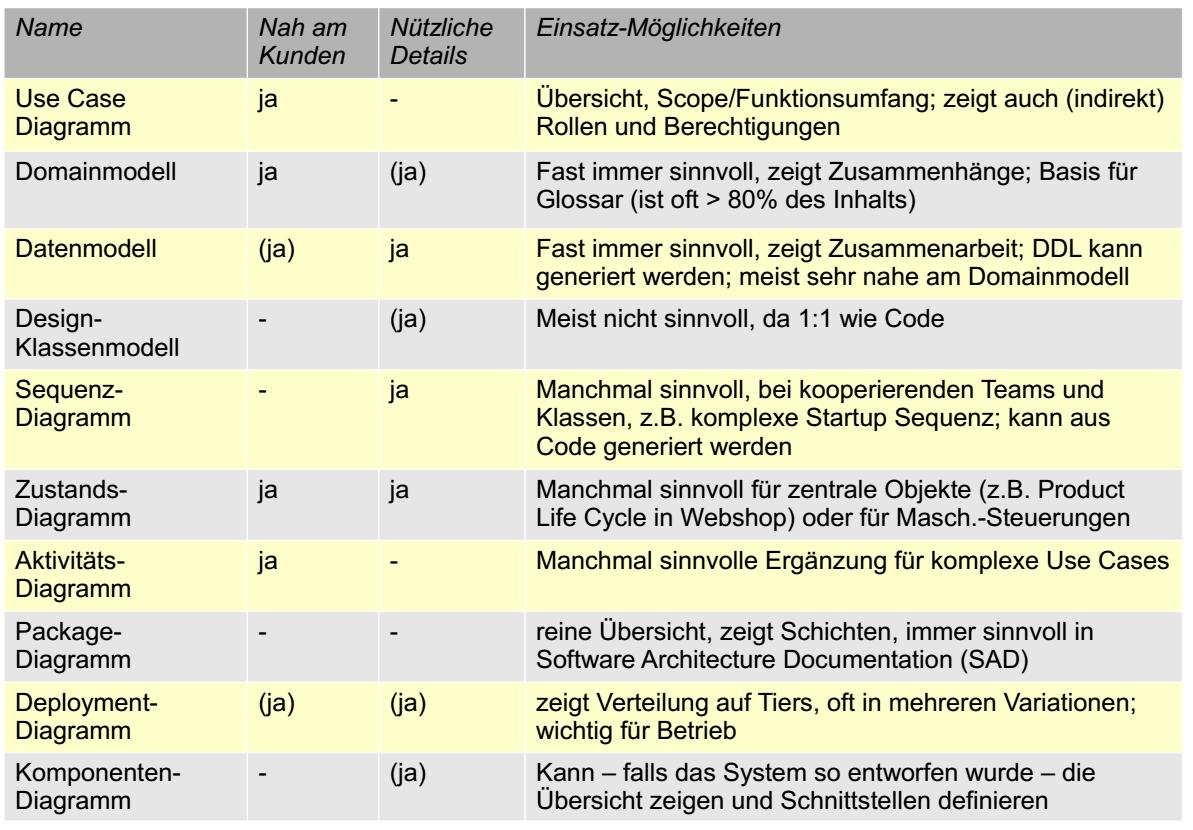
\includegraphics[width=0.9\linewidth]{images/uebersicht_diagramme}
	\caption{Übersicht Diagramme}
	\label{fig:uebersichtdiagramme}
\end{figure}

\clearpage

\subsection{Use Case Diagramm}
Bei Use Case Diagramm muss auf folgende Dinge geachtet werden:
\begin{itemize}
	\item Der Kontext wird als grosses leeres Reckteck abgebildet (Systemkontext)
	\item Akteure werden als Strichmännchen dargestellt
	\item Die Use Cases werden in Ellipsen abgebildet
	\item Include-Beziehungen: Werden mittels \lstinline|<<include>>| gekennzeichnet und mit einer gestrichelten Linie. Sie wird verwendet, wenn ein Use Case einen anderen enthält.
	\item Extend-Beziehungen: Werden mittels \lstinline|<<extend>>| gekennzeichnet und mit einer gestrichelten Linie. Sie wird verwendet, wenn ein Use Case einen anderen erweitert
	\item Externe Systeme werden als Klasse vom Typ \lstinline|<<actor>>| gekennzeichnet
	\item Änderungen an Kundendatensätzen können mit CRUD abgekürzt werden.
\end{itemize}
\begin{figure}[h]
	\centering
	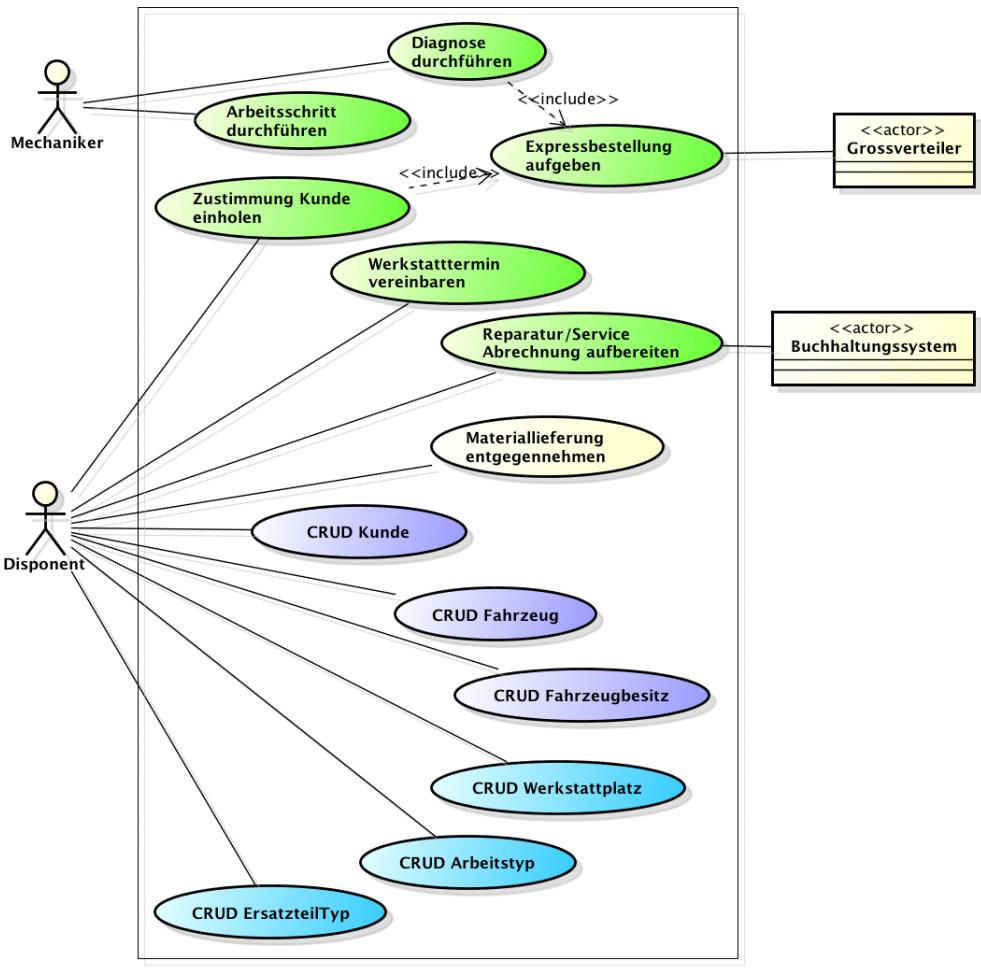
\includegraphics[width=0.7\linewidth]{images/use_case_diagramm}
	\caption{Use Case Diagramm}
	\label{fig:usecasediagramm}
\end{figure}

\clearpage

\subsection{Zustandsdiagramm}
Zustandsdiagramme (State Machine Diagrams) zeigen zustandsabhängiges Verhalten von Systemen. Man kann ein Zustandsdiagramm für einen bestimmten Use Case oder für ein ganzes System erstellen (wird bei komplexen System unübersichtlich). Zustandsdiagramme zeigen die zulässige Reihenfolge aller Systemereignisse.
\begin{figure}[h]
\centering
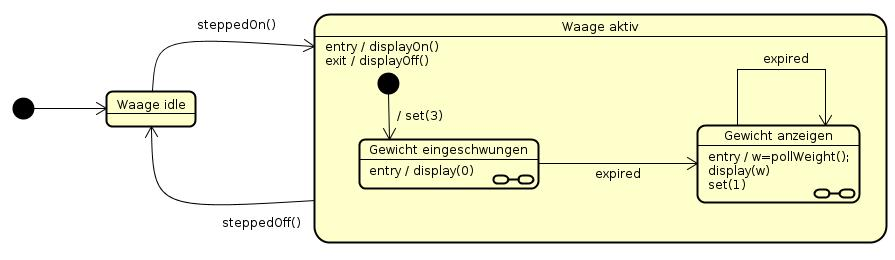
\includegraphics[width=0.7\linewidth]{images/state_machine_diagram}
\caption{Zustandsdiagramm}
\label{fig:statemachinediagram}
\end{figure}

\begin{description}
	\item[Startzustand] Der Startzustand wird mit einem schwarzen vollen Punkt gekennzeichnet
	\item[Endzustand] Der Endzustand ist ebenfalls ein voller Punkt, jedoch mit einem Kreis herum.
	\item[State] Zustand eines Objektes. Ein Zustand hat mehrere Events als Eigenschaft. Hat Start- und End-Zustand
	\begin{itemize}
		\item Entry: Aktion die beim Eintritt ausgeführt wird
		\item Do: Wird während dem State ausgeführt
		\item Exit: Wird beim Verlassen des States ausgeführt
	\end{itemize}
	\item[Nested State] Ist eine genauere Darstellung eines States. Enthält wiederum mehrere States. Hat meistens keinen Endzustand
	\item[Event] Passiert zu einem Zeitpunkt und löst Aktivität aus
	\item[Activity] Das Resultat was ein System macht aufgrund eines Events. (optional)
	\item[Guard] Voraussetzung (optional)
	\item[Transition] Beim Zustandübergang können Activities ausgeführt werden. Er wird nach folgendem Schema beschriftet: \lstinline|event [guard] / activity|. Eine Transition benötigt immer \textbf{mindestens einen Guard oder Event!}
\end{description}

\subsubsection{Vorgehen}
\begin{enumerate}
	\item Relevante	Zustände identifizieren.
	\item Relevante Ereignisse (Events) identifizieren.
	\item Transitionen erfassen.
	\item Guards identifizieren und am richtigen Ort	erfassen.
	\item Aktivitäten identifizieren und am richtigen Ort erfassen.
	\item Diagramm evtl. mittels Nesting vereinfachen
\end{enumerate}

\subsection{Activity Diagramme}
Ein Activity Diagramm zeigt sequentielle und parallele Aktivitäten. Es ist eine Erweiterung des Flussdiagramms. Es wird insbesondere für Geschäftsprozesse und Use Cases mit parallelen Aktivitäten verwendet. Ein Activity Diagramm kann auch in verschiedene Partitionen  unterteilt werden (z.B welche Abteilung erledigt welche Arbeit)

\subsubsection{Nodes}
\begin{description}
	\item[Initial Node] Startpunkt
	\item[Fork Node] Paraleller Ablauf (zwei Token). Ein Fork Node wird wie der Join Node mit einem schwarzen Strich dargestellt.
	\item[Decision Node] Der Token nimmt genau diesen Weg, auf welchen die Bedingung zutrifft
	\item[Merge Node] Fügt eine Decision wieder zusammen
	\item[Join Node] Wartet auf alle Tokens und fügt diese zusammen (Synchronisation)
	\item[Object Node] Das resultierende Objekt einer Action
\end{description}

\begin{figure}[h]
\centering
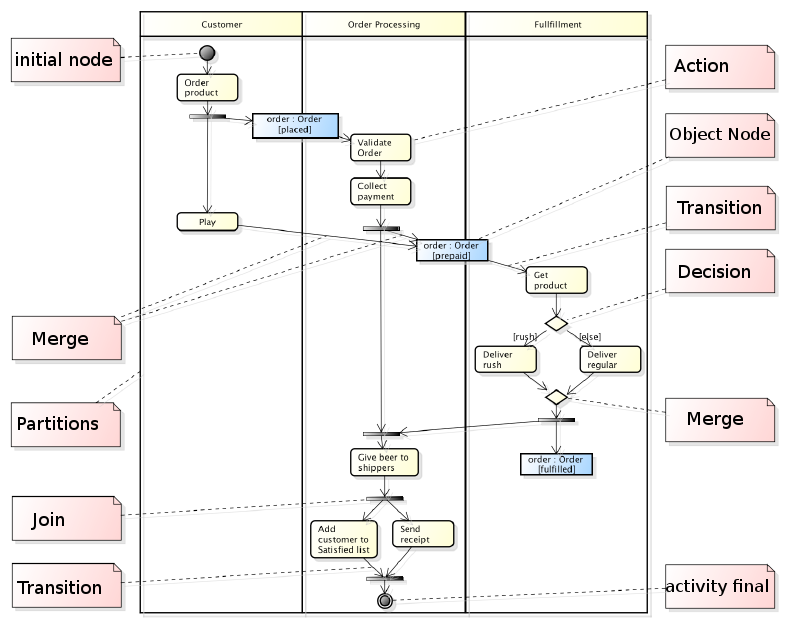
\includegraphics[width=0.8\linewidth]{images/activity_diagram}
\caption{Aktivitätsdiagramm}
\label{fig:activitydiagram}
\end{figure}

\newpage

\subsection{Sequenzdiagramme}
\begin{itemize}
	\item Ein Sequenzdiagram zeigt detailiert das Zusammenspiel von mehreren Klassen, sowie deren Abhängigkeiten. Speziell komplexe Sequenzen können gut erklärt und diskutiert werden.
	\item Man programmiert ohne eine einzige Zeile Code zu schreiben
	\item Bestimmte Enwicklungsumgebungen können SD's zur Laufzeit generieren, was für die Dokumentation recht praktisch ist.
	\item Wie bei allen Diagrammen muss man immer darauf achten, dass die Diagramme aktuell bleiben. Dies ist insbesondere der Fall wenn das Diagramm nahe beim Code ist.
	\item Die Zeit verläuft von oben nach unten. Die dicken Blöcke entsprechen der Zeitdauer, die eine Klasse arbeitet.
\end{itemize}

\subsubsection{Komponenten}
\begin{itemize}
	\item sd: ist das Sequenzdiagramm
	\item alt: Alternative Ablaufe mit Bedingungen. Ist ein \lstinline|if-then-else|
	\item opt: ''Optionaler'' Ablauf mit einer Bedingung (\lstinline|if|)
	\item ref: ist ein Unterprogramm
	\item loop: Wiederhole bis Abbruchbedingung eintritt. Abbruchbedingung wird direkt beim Loop definiert
\end{itemize}

\begin{figure}[h!]
\centering
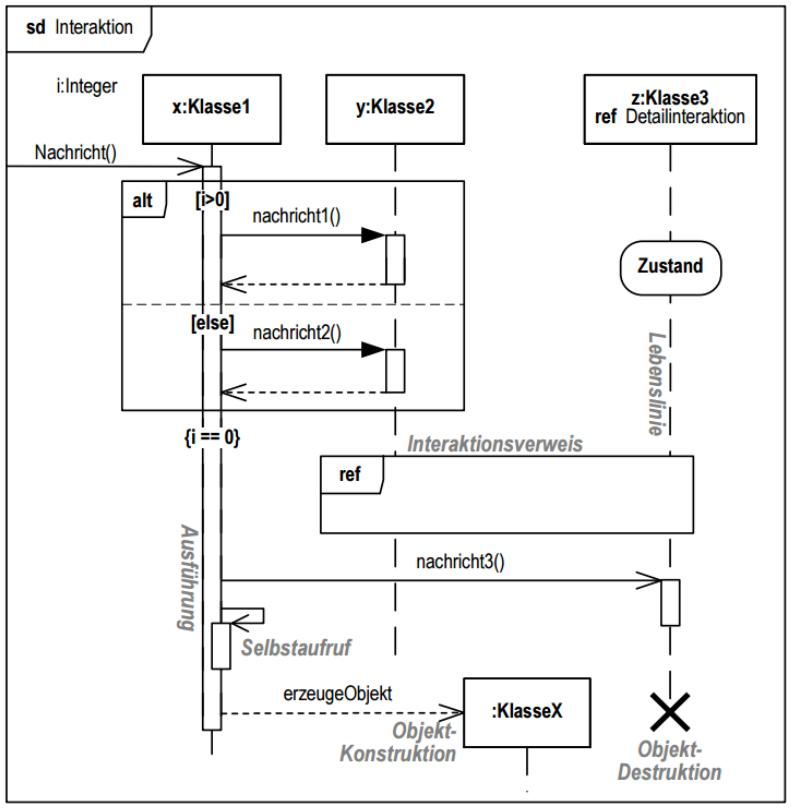
\includegraphics[width=0.55\linewidth]{images/sequencediagram}
\caption{Sequence Diagramm}
\label{fig:sequencediagram}
\end{figure}

\begin{lstlisting}
HouseBlend coffee = new HouseBlend();
Soy soy = new Soy(coffee);
Mocha mocha = new Mocha(soy);
Whip whip = new Whip(mocha);
// call
whip.cost();
\end{lstlisting}

\begin{figure}[h!]
	\centering
	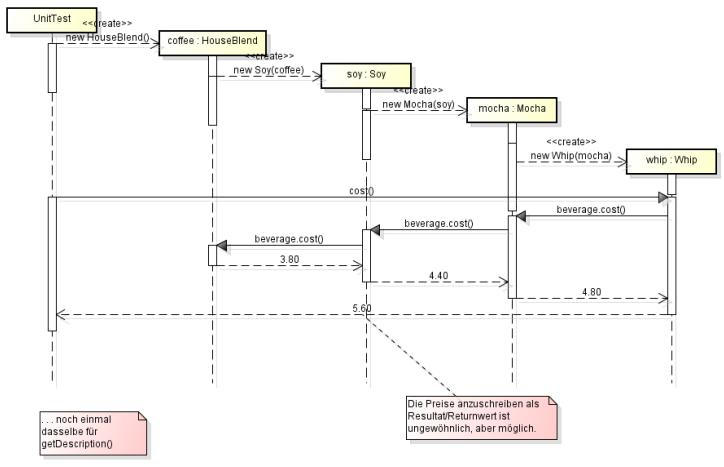
\includegraphics[width=0.9\linewidth]{images/sequence_decorator}
	\caption{Sequenz Diagramm Decorator}
	\label{fig:sequencedecorator}
\end{figure}


\clearpage

\subsection{SSD: System Sequenzdiagramm}
\begin{itemize}
	\item Es gibt immer nur einen Aktor und ein System. Das System ist immer eine Blackbox.
	\item Das SSD modeliert oft ein Use Case Szenario $\rightarrow$ Verweise auf das Main Success Szenario (\textbf{UC-Nummer angeben})
	\item Dass SSD agiert auf einer höheren Abstraktionsbene, wobei der Wille des Benutzers beschrieben wird.

	\item Das SSD wird in der Enwicklung sehr früh erstellt, da es eine vereinfachte Sicht darstellt.
\end{itemize}

\begin{figure}[h]
\centering
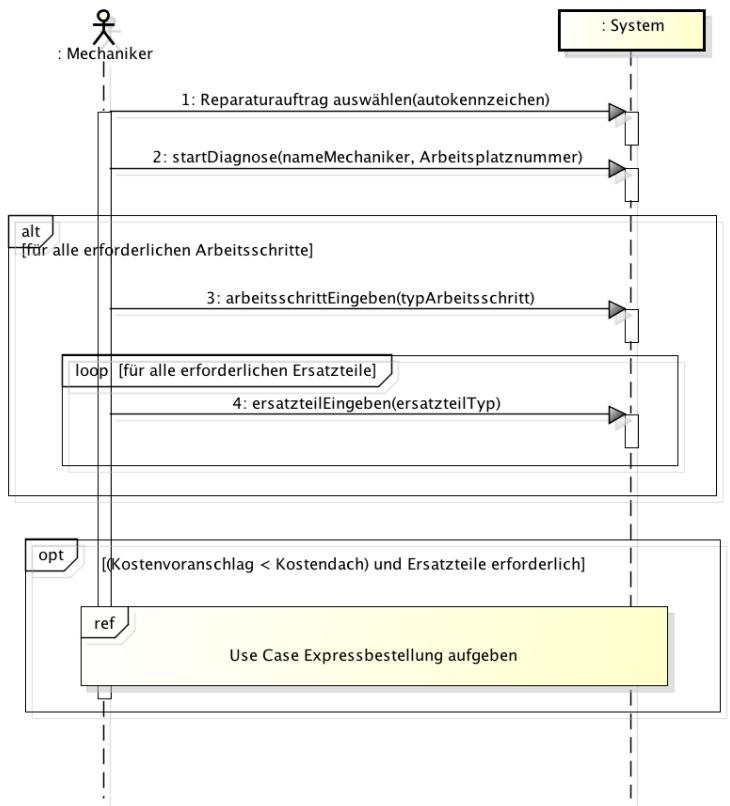
\includegraphics[width=0.6\linewidth]{images/ssd}
\caption{System Sequenzdiagramm}
\label{fig:ssd}
\end{figure}

\clearpage

\subsubsection{Operation Contract}
Ein Operation Contract beschreibt eine Änderung im System, wenn eine Operation durchgeführt wird. Die Operation \textbf{bezieht sich immer auf eine einzige Operation im System Sequence Diagram (SSD)}. Wenn man einen Operation Contract schreibt, sollte man sich den Systemstatus \textbf{vor und nach einer Operation} vorstellen (Snapshots). Diese beiden Zustände müssen beschrieben werden. Es muss nicht aufgezeigt werden, wie die Operation durchgeführt wird, sondern wie das Resultat aussieht.
\begin{itemize}
	\item Name: [Operation Name]
	\item Responsibilities: [Perform a function / Beschreibung Aufgaben dieser Operation]
	\item Cross References: [System functions and Use Cases]
	\item Exceptions: [..]
	\item Preconditions: [Wie sieht das System \textbf{vor} der Änderung aus?]
	\item Postconditions: [Wie sieht das System \textbf{nach} der Änderung aus?]
\end{itemize}

\subsection{Sequenzdiagramm vs SSD}
\begin{table}[h]
	\centering		
	\begin{tabu} to \linewidth {l X X}
		\toprule
		& SSD: System Sequenzdiagramm & Sequenzdiagramm \\
		\midrule
		Was & System Interaktion & Zusammenspiel von mehreren Klassen \\
		Akteure & 2 Dialogpartner & sinnvoll mit mehr als 2 Dialogpartner \\
		Ansicht & Black Box & White Box\\
		Zeitpunkt & Teil von Requirements Analysis & Teil von OOD bzw. nachträgliche Doku\\
		 & Näher beim User/Kunden & Nah beim Code/Entwickler \\
		\bottomrule
	\end{tabu}
	\caption{Multiplitäten}
\end{table}

\clearpage

\subsection{Deployment Diagramme}
\begin{itemize}
	\item Deploymentdiagramme zeigen, welche Software Komponenten auf welchen Knoten (Hardware) laufen.
	\item Oft macht man mehrere Diagramme die verschiedene Szenarien visualisieren (Performance, Security)
	\item Nested Execution Environments: Ausführungs Umgebungen werden typischerweise ineinander geschachtelt
	\item Assoziationen: Verbindung zum Protokoll (evtl. Multiplizitäten)
	\item Die Deployment Diagramme werden vom Server Manager geschrieben und sollten ebenfalls möglichst am Anfang definiert werden.
\end{itemize}

\subsubsection{Bestandteile}
\begin{description}
	\item[Device Node] Zeigt ein Gerät (Server oder Client) an
	\item[Execution Environment Node] Zeigt eine Laufzeitumgebung an. Ist immer in einem Device Node gepackt.
	\item[Artefact] Beschreibt ein Softwareproduct
\end{description}

\begin{figure}[h]
	\centering
	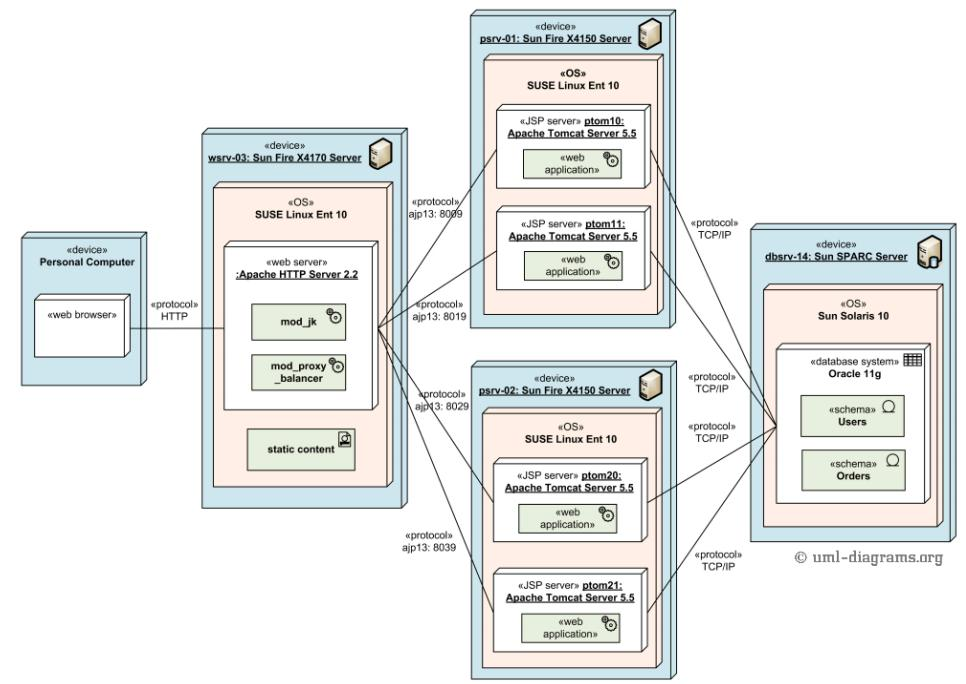
\includegraphics[width=0.6\linewidth]{images/deployment_diagram}
	\caption{Deployment Diagram}
	\label{fig:deploymentdiagram}
\end{figure}

\begin{figure}[h]
	\centering
	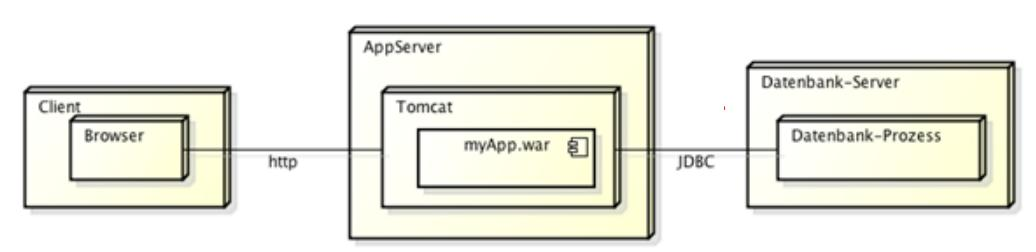
\includegraphics[width=0.6\linewidth]{images/deployment_diagram_simple}
	\caption{Vereinfachtes Deployment Diagram}
	\label{fig:deploymentdiagramsimple}
\end{figure}

\clearpage

\subsection{Packagediagramm}
Das Paketdiagramm ist ein Strukturdiagramm. Es zeigt eine bestimmte Sicht auf die Struktur des modellierten Systems

\subsubsection{Bestandteile}
\begin{description}
	\item[Package] Stellt eine Software Schicht dar
	\item[Dependency] Zeigt die Abhängigkeiten der Packages.
	\item[Merge] Mit dem Keyword \lstinline|<<merge>>| wird angezeigt, dass ein Paket aus mehreren anderen Paketen kombiniert wird.
	\item[Import] Mit dem Keyword \lstinline|<<import>>| wird eine gerichtete Beziehung zwischen zwei Paketen visualiert.
\end{description}
\begin{figure}[h]
	\centering
	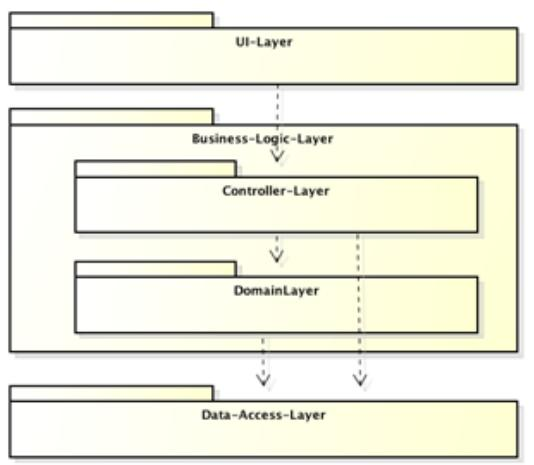
\includegraphics[width=0.7\linewidth]{images/package_diagram}
	\caption{Package Diagram}
	\label{fig:packagediagram}
\end{figure}

\section{Konfigurationsmanagement}
Software Konfigurations Managment ist die Disziplin zur Verfolgung und Steuerung der Evolution von Software. Zum Konfigurationsmanagement gehören vier Teile die miteinander interagieren:

\subsection{Versionskontrolle}
\begin{itemize}
	\item Verwaltet die Änderungen am Sourcecode
	\item Wer hat Wann, Was und Warum so gemacht
	\item Für die Versionskontrolle kommt oft Git oder SVN, CVS zum Einsatz
\end{itemize}

\subsection{Buildmanagement}
\begin{itemize}
	\item Das Buildmanagment beschreibt den Vorgang der Erzeugung von Artefakten aus Software Elementen
	\item Ein Artefakt ist ein Produkt, das als Zwischen- oder Endergebnis in der Softwareentwicklung entsteht
\end{itemize}

\subsection{Releasemanagement}
\begin{itemize}
	\item Das Releasemanagment befasst sich mit dem Veröffentlichen der erzeugten Artefakte
	\item Ebenfalls geht es hier um die Dokumentation und Definition des Installationsvorganges
\end{itemize}

\subsection{Changemanagement}
\begin{itemize}
	\item Das Changemanagement definiert einen geordneten Umgang mit Änderungswüschen und Fehler
\end{itemize}
\begin{figure}[h]
	\centering
	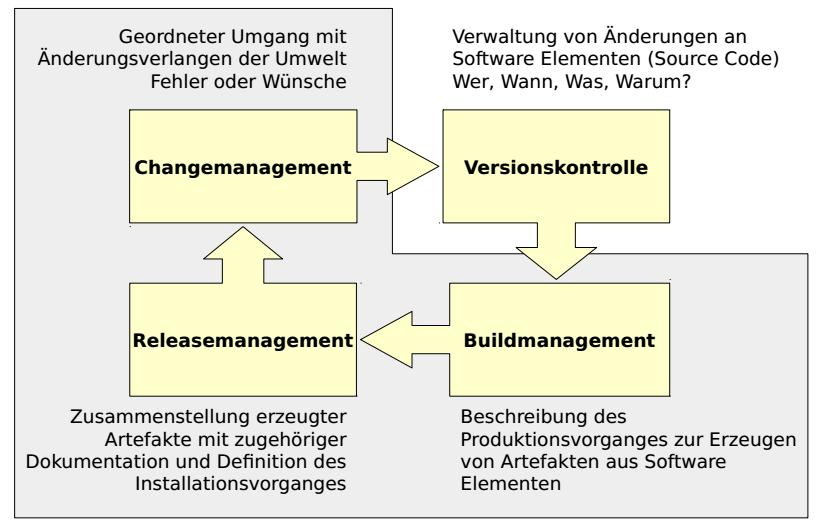
\includegraphics[width=0.7\linewidth]{images/konfigurationsmanagment}
	\caption{Konfigurationsmanagement}
	\label{fig:konfigurationsmanagment}
\end{figure}


\section{Versionskontrolle}
Versionskontrollsysteme (VCS) protokollieren Änderungen an einer oder mehreren Dateien über die Zeit hinweg, so dass man zu jedem Zeitpunkt auf Versionen und Änderungen zugreifen kann. Bekannte Vertreter sind Git, Mercurial, Bazaar, CVS und SVN. Die ersten drei sind \textbf{lokal und dezentral} organisiert und die letzten beiden liegen zentral auf einem Server.

\begin{description}
	\item[Changeset] Inhaltsänderung an einer oder mehreren Dateien
	\item[Commit] Abspeichern eines Changeset im Repository
	\item[Version] Eindeutige Identifizierung eines Commits
\end{description}

\subsection{Merkmale}
\begin{itemize}
	\item Jederzeit ist bekannt, wer, was, warum geändert hat.
	\item Alle Zustände einer Komponente kann nachverfolgt werden
	\item Unbeabsichtigte Änderungen sind ausgeschlossen, da diese explizit durch einen Commit bestätigt werden müssen.
\end{itemize}

\subsection{Commits}
Man sollte oft und früh commiten, sofern folgende Bedingungen erfüllt sind: (\textbf{Commit Early, Commit Often})
\begin{itemize}
	\item Feature funktioniert
	\item Feature hat Tests
	\item Feature ist dokumentiert
	\item Feature wurde gereviewed
\end{itemize}

\subsection{Branches}
Es empfiehlt sich, wenn immer möglich, mit lokalen Branches zu arbeiten und nur fertige Features in den \lstinline|master|-Branch zu mergen.

\subsection{Definition of Done}
\begin{enumerate}
	\item Code übersetzt ohne Fehler und ohne Warnungen
	\item Unit Tests laufen fehlerfrei
	\item Test-Abdeckungsgrad wie definiert (in sep. Doku)
	\item Kein unaufgeräumter (z.B. auskommentierter) Code
	\item Alles Unfertige ist markiert mit \lstinline|TODO:|
	\item Code ist wo nötig, und richtig mit Kommentaren versehen
	\item metrics, findbugs, ReSharper, structure101, STAN und andere 
	eingesetzte Analysetools geben grünes Licht
	\item Vier-Augen-Prinzip: entweder Pair Programming oder gereviewt und 
	Review dokumentiert
\end{enumerate}


\subsection{Git}
Git ist eine Versionsverwaltung. Erzeugte Dateien wie z.B *.pdf oder *.exe sollte nie in einem Repo abgelegt werden.
\begin{figure}[h]
	\centering
	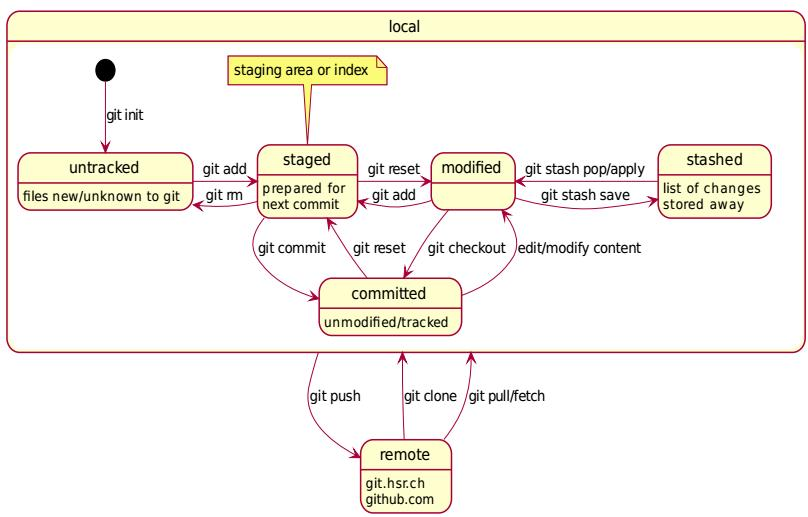
\includegraphics[width=0.9\linewidth]{images/git_overview}
	\caption{Git Übersicht}
	\label{fig:gitoverview}
\end{figure}

\subsubsection{Struktur}
\begin{description}
	\item[Master] Hauptstamm
	\item[Branch] Abzweigung vom Stamm
	\item[HEAD] Zeiger auf den aktuellsten Commit des aktuellen Branches. Kann mit \lstinline|checkout| versetzt werden.
	\item[Tag/Label] Eindeutiger Name für bestimmten Commit
\end{description}

\subsubsection{Branches}
Es empfiehlt sich, wenn immer möglich, mit lokalen Branches zu arbeiten.
\begin{enumerate}
	\item Feature Branch erstellen
	\item Änderung durchführen
	\item Feature in Branch überführen (mittels Merge oder Rebase). Rebasing ist dem Merging vorzuziehen, da man damit eine saubere History erreicht. ACHTUNG: Falls sonst jemand auf dem gleichen Branch arbeitet, sollte kein Rebase gemacht werden.
	\item Branch löschen
\end{enumerate}

\subsubsection{Operationen}
\begin{description}
	\item[Einrichten]  \hfill
	\begin{description}
		\item[git config --global user.name ''''] Username setzen
		\item[git config --global user.email ''''] Email setzen
	\end{description}
	\item[Basisoperationen] \hfill
	\begin{description}
		\item[git clone https://github.com/xxx/yyy.git] Entferntes Repository kopieren
		\item[git init] Erstelle ein lokales Git Repository
		\item[git add file.txt] Füge file.txt in die Versionkontrolle (staged). Mit dem Flag -p kann selektiv hinzugefügt werden.
		\item[git reset file.txt] Entfernen aus dem staged Bereich
		\item[git rm --cached file.txt] Entfernen aus dem tracked Bereich. Mit dem Flag -p kann selektiv entfernt werden. Das --cached bewirkt, dass das File nicht im Filesystem gelöst wird.
		\item[git commit -m "Message"] Commit staged changes
	\end{description}
	\item[Remotes] \hfill
	\begin{description}
		\item[git remote add origin https://github.com/xxx/yyy.git] Remote hinzufügen
		\item[git remote show -v] Remotes anzeigen
		\item[git checkout origin/<Commit Hash|Branch|HEAD>] Entfernten Branch auschecken
		\item[$\text{git fetch origin [[remote branch]:[local branch]]}$] Änderungen des entfernten Repositoy abholen.
		\item[$\text{git pull origin [[remote branch]:[local branch]]}$] Pull from remote. Entspricht fetch \& merge
		\item[$\text{git push origin [[local branch]:[remote bra nch]]}$] Push to remote. Mit dem Parameter -u wird der verwendete Remote gespeichert. 
	\end{description}
	\item[Abfragen] \hfill
	\begin{description}
		\item[git status] Beschreibung
		\item[git version file.txt] Beschreibung
		\item[git diff HEAD] Vergleiche aktuelle Änderungen mit dem letzten Commit
		\item[git diff -b -w --staged] Zeige was sich gerade geändert hat. (Ignore blanks and whitespaces)
		\item[git log] Zeit Commit Hashes an
	\end{description}
	\item[Auschecken] \hfill
	\begin{description}
		\item[$\text{git checkout [Commit Hash|Branch|HEAD]}$ ] Commit, Branch oder HEAD auschecken
		\item[git checkout <Commit Hash|Branch|HEAD>\textasciicircum] Gehe eine Commit zurück
		\item[git checkout <Commit Hash|Branch|HEAD>\textasciitilde<Anzahl>] Gehe eine bestimmte Anzahls an Commits zurück
	\end{description}
	\item[Mergen] \hfill
	\begin{description}
		\item[git checkout master] Branch auschecken, in welchen gemerged werden soll
		\item[git merge mybranch] Merge mybranch in den aktuellen Branch
	\end{description}
	\newpage
	\item[Branches] \hfill
	\begin{description}
		\item[git checkout -b branch] Branch erstellen und zu ihm wechseln
		\item[git checkout mybranch] Zu existierendem Branch wechseln
		\item[git branch -d mybranch] Branch löschen
		\item[git branch -f <Commit Hash|Branch|HEAD> <Commit Hash|Branch|HEAD>] Kopiere den einen Branch in einen anderen
		\item[git reset HEAD\textasciitilde1] Branch auf den letzen Commit zurücksetzen
		\item[git revert HEAD] Remote Branch zurücksetzen 
	\end{description}
	\item[Rebase] \hfill
	\begin{description}
		\item[git rebase master mybranch] Packe Branch vor den Master
	\end{description}
	\item[Cherry Pick] \hfill
		\begin{description}
			\item[git cherry-pick C1 C2 C3] Füge einzelne Commit vor den HEAD ein
			\item[git rebase -i Branch] Es öffnet sich ein interaktives GUI in welchem die Commits ausgewählt werden können.
		\end{description}
	\item[Tags] \hfill
		\begin{description}
			\item[git tag descr branch] Erstelle Tag für Branch mit Beschreibung
		\end{description}
	\item[Stashes] \hfill
	\begin{description}
		\item[git stash] Aktueller Stand in Zwischenablage kopieren
		\item[git stash list] Stashes anzeigen		
		\item[git stash apply stash@{1}] Bestimmte Stash von der Zwischenablage zurückkopieren. \lstinline|git stash pop| nimmt einfach den letzten Stash vom Stack
	\end{description}
\end{description}

\section{Software Testing}
\subsection{Terminologie}
\begin{description}
	\item[SUT: System under Test] Das zu testende System
	\item[Validierung] Machen wir das Richtige (Anforderungen spezifizieren)
	\item[Verfikation] Machen wir es richtig (Systemtests, Integrationstests, Unit Tests)
\end{description}

\subsection{Ablauf}	
\begin{description}
	\item[1. Testplan] Wer, was, wann, wie?
	\item[2. Testspezifikation] Beschreibt was getestet werden muss
	\item[3. Testprotokoll] Beschreibt das Resultat der Tests
\end{description}

\begin{figure}[h!]
	\centering
	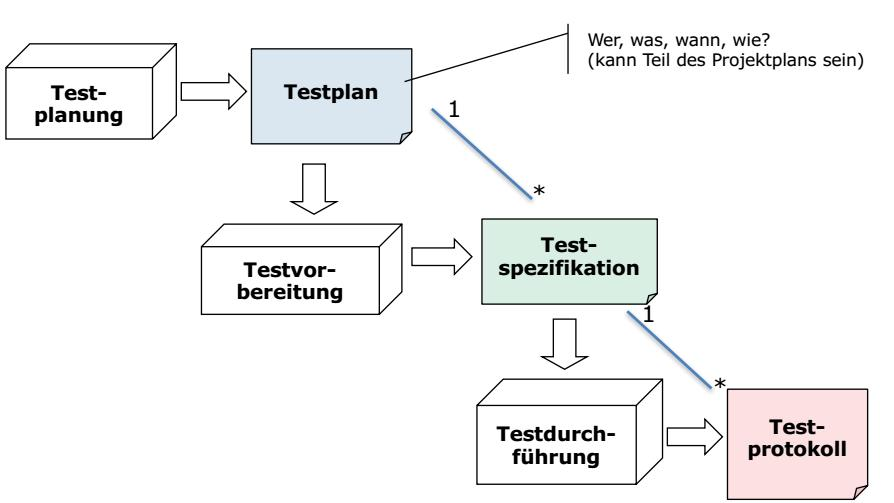
\includegraphics[width=0.45\linewidth]{images/testing}
	\caption{Ablauf einer Tests}
	\label{fig:testing}
\end{figure}

\subsection{Testfälle}
Gute Testfälle sind, \lstinline|null|, negative Werte, leere Strings, ungültige Eingaben
\begin{figure}[h!]
	\centering
	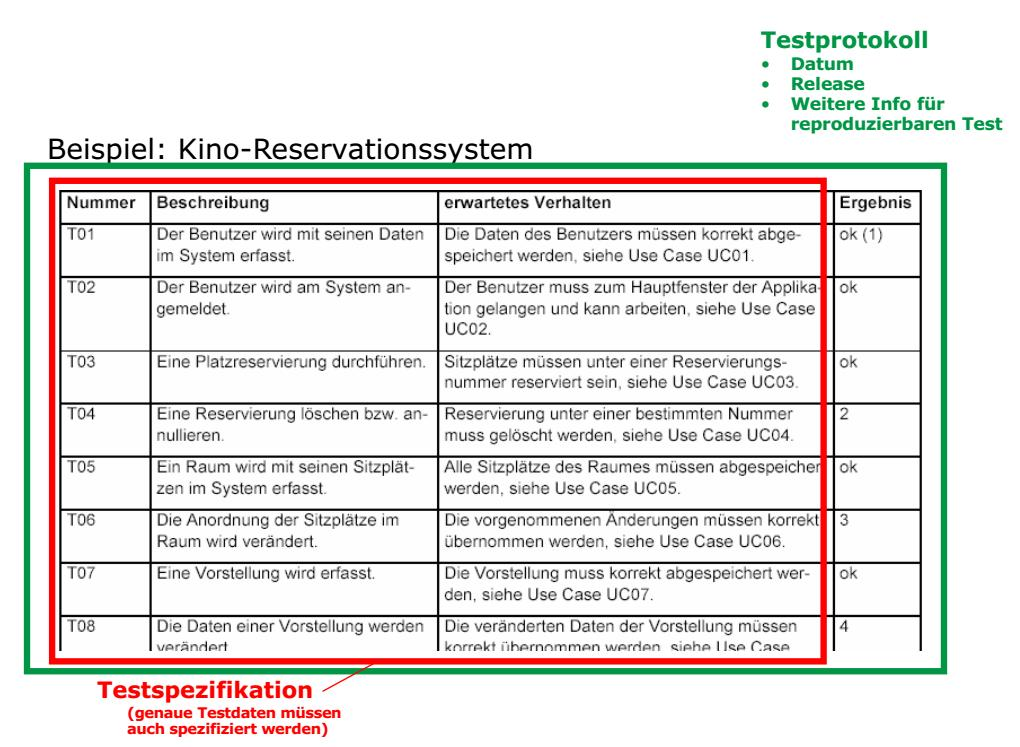
\includegraphics[width=0.5\linewidth]{images/testspec_protocol}
	\caption{Testspezifikation und Protokoll}
	\label{fig:testspecprotocol}
\end{figure}

\subsection{Vorgehen}
\begin{enumerate}
	\item Früh testen
	\item Häufig testen
	\item Systematisch testen
	\item Automatisiert testen: 
	\item Test anything that might break: Keine Tests für funktionslosen Code
	\item Test everything that does break: Test schreiben, der den Fehler reproduziert, danach korrigieren (Regressionstests)
	\item New Code is guilty until proven innocent
	\item Tests ausführen, vor dem einchecken (am besten automatisiert)
\end{enumerate}


\subsection{Varianten}
\begin{description}
	\item[Modul-, Unit und Microtests] testen die korrekte Arbeitsweise einer einzelnen Klasse/Methode
	\item[Integrationstests] testen das korrekte Zusammenspiel von mehreren Einheiten
	\item[Systemtests] testen das Gesamtsystem nach der Erfüllung der geforderten Anforderungen
	\item[Abnahmentests] Der Kunde testet das Gesamtsystem
\end{description}
\begin{figure}[h]
\centering
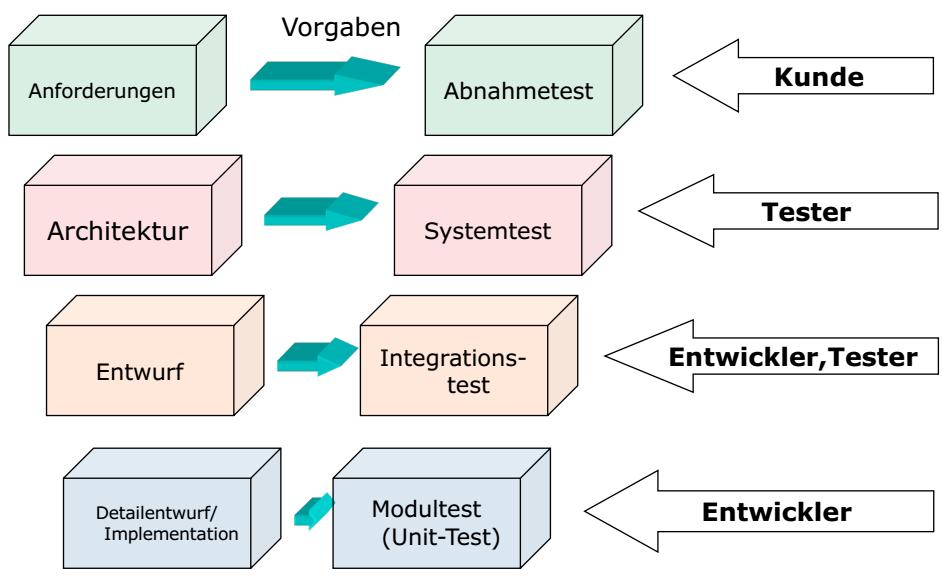
\includegraphics[width=0.7\linewidth]{images/test_varianten}
\caption{Testvarianten}
\label{fig:testvarianten}
\end{figure}


\clearpage

\subsection{Funktionale Tests}
\begin{description}
	\item[Black Box Tests] Testfälle ohne Kenntnis der inneren Struktur. Die Menge der zu testenden Objekte sollte in Äquivalenzklassen unterteilt werden. Danach testet man am besten an den \textbf{Grenzen der Äquivalenzklassen}. (Grenzwertanalyse)
	\item[White Box Tests] Testfälle mit Kenntnis der inneren Struktur (Unit Tests)
\end{description}

\subsection{Nichtfunktionale Tests}
Nichtfunktionale Anforderungen werden mit folgenden Tests überprüft.
\begin{itemize}
	\item Usability Tests
	\item Performance Messungen
\end{itemize}

\subsection{Automatisierte Tests}
\begin{itemize}
	\item Der grosse Vorteil von automatisierten Tests ist, dass sie wiederholbar sind
	\item Der Nachteil ist natürlich, dass man mehr Code schreiben muss. Es lohnt sich aber.
\end{itemize}


\subsection{Gute Tests}
Gute Tests folgen dem A-TRIP-Prinzip (Automatic, Thorough, Repeatable, Independent, Professional). Ein guter Test...
\begin{itemize}
	\item Ist systematisch, wiederholbar und automatisiert
	\item Tested genau einen Execution Path 
	\item Tested relevant Dinge (keine Getter und Setter) 
	\item Abhängigkeiten werden durch Mocks ersetzt (Low Coupling)
	\item Folgt dem Arrange, Act, Assert, Teardown Prinzipt
\end{itemize}

\subsection{Äquivalenzklassen}
Äquivalenzklassen sind Wertebereiche für Eingabeparameter eines Tests, für welche ein gleichartiges Verhalten des Prüflings erwartet wird.

\subsection{Failure und Errors}
\begin{description}
	\item[Failure] Beschreibt einen Assert, der fehlschlägt
	\item[Error] Beschreibt eine nicht behandelte Exception im zu prüfenden Code
\end{description}

\subsection{Regressionstests}
Unter einem Regressionstest versteht man in der Softwaretechnik die Wiederholung von Testfällen, um sicherzustellen, dass Modifikationen in bereits getesteten Teilen der Software keine neuen Fehler verursachen. Man schreibt dazu, für jeden gefundenen Bug einen Test, der den Fehler reproduziert.

\clearpage

\subsection{Microtest}
Microtests sind kurze, einfache, automatisierte Tests die \textbf{genau ein Verhalten} eines Objekts überprüfen. Dabei sollte so viele ''Execution Paths'' wie möglich abgedeckt werden. Microtests werden in drei Dimensionen gemessen. Bevor man mit Test Driven Developement anfängt, sollte man sich mit kleiner Komplexität, geringen Abhängigkeiten und After-Testing beschäftigen.
\begin{description}
	\item[Complexity, Komplexität:] Die Komplexitätsachse geht von einfach bis hart
	\item[Collaboration, Abhängigkeiten:] Haben die Klassen grosse oder kleine Abhängigkeiten untereinander
	\item[Timing, Zeitpunkt:] Schreiben wir die Tests vor oder nachdem wir den Code geschrieben haben
\end{description}

\begin{figure}[h]
\centering
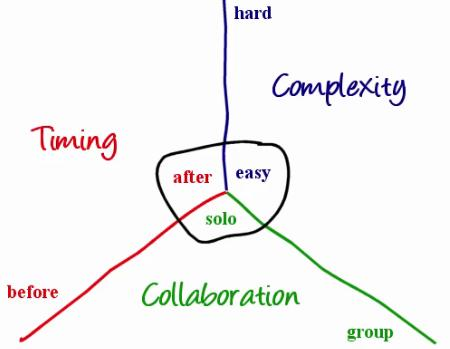
\includegraphics[width=0.4\linewidth]{images/microtest}
\caption{Microtest Dimensionen}
\label{fig:microtest}
\end{figure}

\subsubsection{Ablauf}
Ein Microtest besteht immer aus folgender Abfolge:
\begin{enumerate}
	\item Arrange: Die zu testenden Objekte instanzieren
	\item Act: Die zu testende Funktionalität aufrufen
	\item Assert: Definiere das erwartete Resultat und vergleiche den Rückgabewert mit diesem
	\item Teardown: Aufräumen, sofern dies nicht vom Garbage Collector erledigt wird.
\end{enumerate}

\clearpage

\subsection{jUnit}
JUnit Tests sollten im gleichen Package wie der Production Code sein, jedoch in separierten Order.
\begin{itemize}
	\item myProject/src (ch.hsr.mypackage)
	\item myProject/tests (ch.hsr.mypackage)
\end{itemize}

\begin{lstlisting}
import static org.junit.Assert.*;

public class MyTestClass {
	private List<String> myList;
	
	@BeforeClass
	public static void openSession() {
		openDBConnection(); // rather time consuming, so do it just once
	}
	
	@Before
	public void setUp() { 
		list = new ArrayList<>();
	}

	@Test
	public void myTest() { 
		myList.add("test");
		assertEquals("test", myList.get(0))
	}
	
	@After
	public void tearTown() {
		myList.clear();
	}
	
	@AfterClass
	public static void closeSession() {
		closeDBConnection();
	}
}

// Asserts
assertEquals(expected, actual);
assertEquals(expected, actual, precision); // float, double
assertSame(anObject, sameObject);
assertNull(object);
assertNotNull(object); 

// Exceptions: Expected Annotation
@Test(expected=NumberFormatException.class)
public void parseIntThrowsException() { ... }
// Exceptions: Fail explicit
public void testParseIntThrowsException() {
	try {
		Integer.parseInt("trying to parse letters instead of numbers");
		fail("Should have thrown NumberFormatException"); // should not happen
	} catch (NumberFormatException expectedException) {
		// if we get here it means the test has passed
	}
}

\end{lstlisting}

\section{Clean Code}
\subsection{Regeln}
\paragraph{Gutes Naming}
\begin{itemize}
	\item Aussprechbar (besser \lstinline|powersOfTwo| anstatt \lstinline|pwrsOf2|), konsistent, mit klarer Bedeutung (nicht text1, text2, text3)
	\item Methoden sind immer Verben
	\item boolean starten mit ''is''
	\item Kurze Namen nur bei kleinen Scope/Gültigkeitsbereich einer Variable/Methode
	\item Nicht abkürzen wenn man nur 3 Buchstaben spart (z.B groupID, grpID oder nameLength, namln)
	\item keine Präfixe
	\item Keine Zahlen, Umlaute verwendent
	\item Keine anonymen Konstanten (Ausnahme 0 und 1). z.B \lstinline|for(int i = 1; i < 27; i++;)| $\rightarrow$ \lstinline|const int MAX_OPEN_FILES = 27;|
\end{itemize}
\paragraph{Nützliche Kommentare}
\begin{itemize}
	\item Der Methodenname sollte sagen, was gemacht wird
	\item Die Statements im Code zeigen, wie es gemacht wird
	\item Ein (eventueller) Kommentar sollte erklären warum es genau so gemacht wird.
	\item Ein Kommentar sollte nie das offensichtliche kommentieren
	\item Kommentare wirklich nur wenn nötig schreiben
	\item JavaDoc sollte nur auf den unteren Schichten geschrieben werden, damit die überliegenden Layer klar verständlich sind, ohne den Code zu lesen.
\end{itemize}
\paragraph{Programmiere für den Menschen, nicht für den Compiler}
\begin{itemize}
	\item Code wird häufiger gelesen als geschrieben
	\item Der Code sollte so geschrieben werde, wie wir ihn selber gerne antreffen würden. 
	\item Ein Review in der Gruppe zeigt, ob der Code gut lesbar ist.
	\item Weiter gehen als ''Hurra es läuft'' oder ''Works for me''
\end{itemize}
\paragraph{DRY: Don't Repeat Yourself}
\begin{itemize}
	\item Kein duplizierter Code
	\item Bei viel Copy Paste, wird der Code aufgebläht und es entstehen mehr Fehler, Arbeit bei Änderungen
	\item Auch bekannt als DIE: Duplicate is Evil
\end{itemize}
\paragraph{Single Responsibility Principle}
\begin{itemize}
	\item Eine Methode ist genau für eine Sache zuständig.
	\item Dieses Paradigma ist auch bei Klassen sinnvoll, jedoch schwerer umzusetzen.
	\item Wird die Single Responsibility verletzt, hat dies Folgen bei Git, Unit Tests und Kopplung steigt.
\end{itemize}
\paragraph{KISS: Keep It Simple Stupid}
\begin{itemize}
	\item Es ist schwerer, den Programmcode einfach zu halten, anstatt ihn komplex zu programmieren.
	\item Beim Testen wird schnell klar, ob ein Code einfach ist.
\end{itemize}
\paragraph{YAGNI: You Ain't Gonna Need it}
\begin{itemize}
	\item Es sollte nichts entwickelt werden, ohne dass eine explizite Anforderung dafür besteht.
	\item Keine Implementierung im Sinne ''In der Zukunft könnte man das brauchen''.
\end{itemize}
\paragraph{Programm to the Interface, not Implementation}
\begin{itemize}
	\item \lstinline|List<T>| anstatt \lstinline|ArrayList<T>|
\end{itemize}
\paragraph{Isolte What Changes}
\begin{itemize}
	\item Alles was sich nicht ändert, soll in einem Interface modelliert werden
\end{itemize}
\paragraph{Aufgeräumter Coder}
\begin{itemize}
	\item Einrückung, Formatierung ist für die Übersicht wichtig
	\item Auskommentierter Code sollte weggelassen werden. Dafür gibt es Version Control
	\item TODO's implementieren
	\item Geschweifte Klammern immer setzen (insbesondere bei Verschachtelungen)
\end{itemize}
\paragraph{Positive Bedingungen}
\begin{itemize}
	\item Im \lstinline|if| sollten immer die positiven Bedingen deklariert werden
	\item Ausnahme sind die Guards. Ein Guard lässt eine Methode schnell terminieren, falls bestimmte Bedinungen nicht gegeben sind.
	\item Ein schneller Ausstieg ist auch, wenn z.B eine Iteration bei einem Match frühzeitig abgebrochen werden
\end{itemize}
\paragraph{Coding Guidlines}
\begin{itemize}
	\item Man sollte so programmieren, wie man dies im Team abgemacht hat. Die Konvention kann von der Programmiersprache und der Präferenz des Mehrheit abhängen.
\end{itemize}
\paragraph{Handhabbare Grössen}
\begin{itemize}
	\item Design Diagramme: max A3
	\item Code Breite: max 120 Zeichen
	\item Verschachtelungen: max. 5 Stufen
	\item Methoden: max 30 Zeilen
	\item Klassen: max 300 Zeilen
	\item Tiers: max. 4 Tier
\end{itemize}
\paragraph{No Errors, No Warnings}
\begin{itemize}
	\item Warnungen sollten immer behoben werden, da sich diese ansonsten schnell ansammeln und nie mehr gefixt werden.
	\item Ausnahme: Serializeable UID $\rightarrow$ Compiler so einstellen, dass es die Warnungen ignoriert
	\item Gilt auch für Addons wie Checkstyle, Metrics, FindBugs etc.
\end{itemize}
\paragraph{Kopplung und Kohäsion} \hfill \\
In der Software Enwicklung strebt man immer nach \textbf{High Cohesion UND Low Coupling}. 
\begin{itemize}
	\item Kopplung: Wie stark ist eine Klasse Abhängig von vielen anderen Klassen. Aufrufe von einer Klasse zu anderen, von einem Package zum anderen
	\item Kohäsion: Zusammenhalt innerhalb einer Klasse. Kohäsion soll gegeben sein, sonst gehören die Dinge nicht ein eine Klasse/Package.
\end{itemize}
\paragraph{Smart Data Structures}
\begin{itemize}
	\item Es ist viel wichtiger die richtige Datenstruktur zu verwenden, als wie die Datenstruktur verwendet wird.
	\item z.B gilt bei einer Schweizer Grossbank die Faustregel: \lstinline|2:5:20| (ca. 2 Jahre hält das GUI, 5 Jahre hält die Geschäftslogik und 20 Jahre halten die Daten). Daher sollte die Datenstruktur gut gewählt werden.
\end{itemize}


\section{Patterns}
Die meisten der folgenden Pattern wurden von der Gang of Four (Erich Gamma, Richard Helm, Ralph E. Johnson und John Vlissides) entworfen. Pattern sind \textbf{Best Practice Beispiele}, welche die Kommunikation unter Software Entwickler erleichert. Mit dem gemeinsamen Pattern Vokabular lässt sich \textbf{mit wenig, mehr sagen}. Charakteristik, Qualität und Einschränkungen sind auf anhin klar. Man unterscheidet zwischen drei Varianten von Pattern:

\paragraph{Creational Pattern} \hfill
\begin{itemize}
	\item Abstract Factory \ref{sec:abstractfactory}
	\item Factory Method \ref{sec:factorymethod} ($\surd$)
	\item Singleton \ref{sec:singleton} ($\surd$)
\end{itemize}

\paragraph{Structural Pattern} \hfill
\begin{itemize}
	\item Adapter \ref{sec:adapter} ($\surd$)
	\item Facade \ref{sec:facade} ($\surd$)
	\item Use Case Controller \ref{sec:usecasecontroller} ($\surd$)
	\item Composite \ref{sec:composite} ($\surd$)
	\item Decorator \ref{sec:decorator} ($\surd$)
	\item Proxy \ref{sec:proxy} 
\end{itemize}

\paragraph{Behavioral Pattern} \hfill
\begin{itemize}
	\item Command \ref{sec:command} ($\surd$)
	\item Null Object \ref{sec:nullobject} ($\surd$)
	\item Observer \ref{sec:observer} ($\surd$)
	\item State \ref{sec:state} ($\surd$)
	\item Strategy \ref{sec:strategy} ($\surd$)
	\item Template Method \ref{sec:templatemethod} ($\surd$)
	\item Iterator \ref{sec:iterator}
\end{itemize}

\paragraph{Combined Pattern} \hfill
\begin{itemize}
	\item MVC \ref{sec:mvc} ($\surd$)
\end{itemize}
\clearpage

\subsection{Abstract Factory}
\label{sec:abstractfactory}
Das Abstract Factory Pattern bietet eine Schnittstelle zum Erstellen von Familien verwandter oder zusammenhängender Objekte an, ohne konkrete Klassen anzugeben.
\begin{itemize}
	\item Im Gegensatz zum Factory Method Pattern sollte die Abstract Factory verwendet werden, wenn der Client eine ganze Familie zusammengehörenden Produkten verwenden muss.
	\item Die Abstract Factoy stützt sich auf Objekt Komposition. Die Objekt-Erstellung ist in Methoden implementiert, die in der Fabrik Schnittstelle vorgegeben werden muss.
\end{itemize}

\begin{figure}[h]
\centering
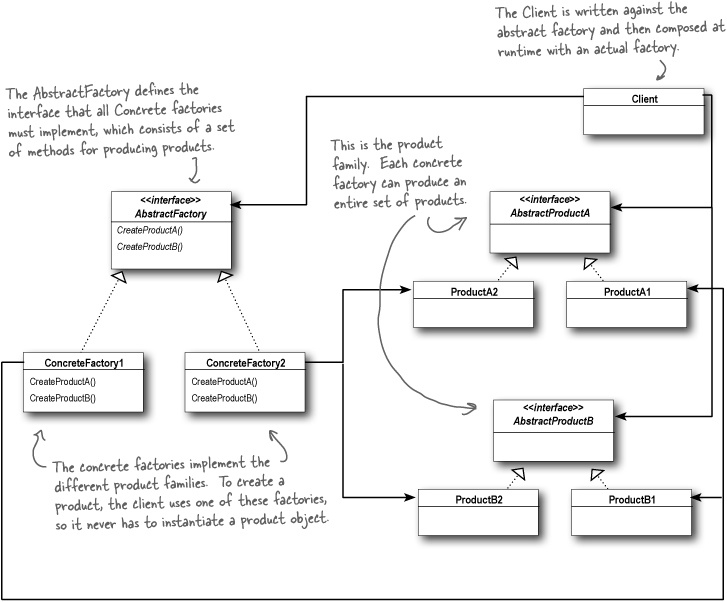
\includegraphics[width=0.7\linewidth]{images/abstract_factory_pattern}
\caption{Abstract Factory}
\label{fig:abstractfactorypattern}
\end{figure}

\newpage


\subsubsection{Implementierung}
\begin{lstlisting}
// abstract product A
public interface Shape {
	void draw();
}

// concrete product A
public class Rectangle implements Shape {
	@Override
	public void draw() {
		System.out.println("Inside Rectangle::draw() method.");
	}
}

// concrete product A
public class Square implements Shape {
	@Override
	public void draw() {
		System.out.println("Inside Square::draw() method.");
	}
}

// abstract product B
public interface Color {
	void fill();
}
// concrete product B
public class Red implements Color {
	@Override
	public void fill() {
		System.out.println("Inside Red::fill() method.");
	}
}
// concrete product B
public class Green implements Color {
	@Override
	public void fill() {
		System.out.println("Inside Green::fill() method.");
	}
}

// abstract factory
public abstract class AbstractFactory {
	abstract Color getColor(String color);
	abstract Shape getShape(String shape) ;
}

// concrete factory A
public class ShapeFactory extends AbstractFactory {

	@Override
	public Shape getShape(String shapeType){
		if(shapeType == null){
			return null;
		}		
		if (shapeType.equalsIgnoreCase("RECTANGLE")){
			return new Rectangle();
		} else if(shapeType.equalsIgnoreCase("SQUARE")){
			return new Square();
		}
		return null;
	}
	
	@Override
	Color getColor(String color) {
		return null;
	}
}

// concrete factory B
public class ColorFactory extends AbstractFactory {
	@Override
	public Shape getShape(String shapeType){
		return null;
	}
	
	@Override
	Color getColor(String color) {
		if(color == null){
			return null;
		}		
		if(color.equalsIgnoreCase("RED")){
			return new Red();	
		} else if(color.equalsIgnoreCase("GREEN")){
			return new Green();
		}
		return null;
	}
}

// producer for the client
public class FactoryProducer {
	public static AbstractFactory getFactory(String choice){
		if(choice.equalsIgnoreCase("SHAPE")){
			return new ShapeFactory();
		} else if(choice.equalsIgnoreCase("COLOR")){
			return new ColorFactory();
		}
		return null;
	}
}

// client
AbstractFactory shapeFactory = FactoryProducer.getFactory("SHAPE");
Shape shape1 = shapeFactory.getShape("CIRCLE");
\end{lstlisting}


\clearpage


\subsection{Factory Method}
\label{sec:factorymethod}
Das Factory Method Pattern definiert eine Schnittstelle zur Erstellung eines Objekts, lässt aber die Unterklassen entscheiden, welche Klassen instantiiert werden. Factory Method ermöglicht einer Klasse, die Instantiierung in Unterklassen zu verlagern.
\begin{itemize}
	\item Das Factory Method Pattern wird verwendet, wenn man eine \textbf{komplexe Erzeugungslogik} hat. Die Logik der Objekterstellung liegt dabei in der Childklasse.
	\item Die Erzeugungslogik wird in dieser Methode gekapselt. Anhang von Parameter wird entschieden wie eine konkrete Klasse erzeugt wird
	\item Typische Methodennamen sind \lstinline|createX()|, \lstinline|makeX()| oder \lstinline|newX()|
	\item Die Faktory Methode darf \textbf{nicht statisch} sein, da die Child die Methode überschreiben müssen. Statische Methoden können auch nicht \lstinline|abstract| sein
\end{itemize}

\begin{figure}[h]
	\centering
	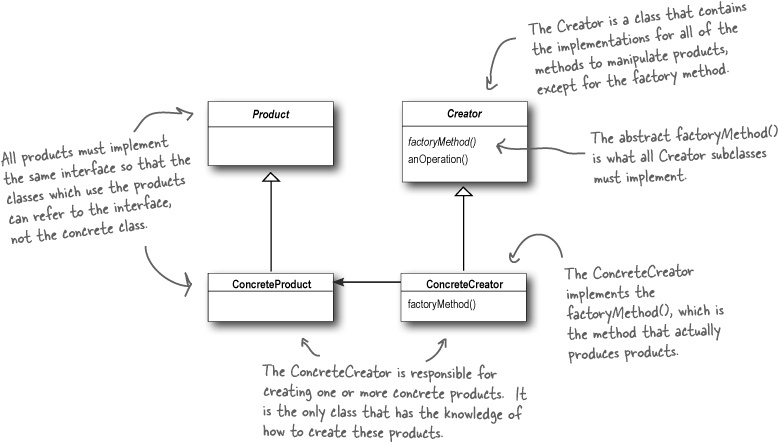
\includegraphics[width=0.9\linewidth]{images/factory_method_pattern}
	\caption{Factory Method}
	\label{fig:factorymethodpattern}
\end{figure}

\clearpage

\subsubsection{Implementierung}
\begin{lstlisting}
public abstract class Creator {
	
	public Product getProduct() {
		
		// create a pizza and execute actions like prepare, bake, cut, ..
		Product product = factoryMethod(type);
		product.x();
		product.y();
		
		return product;
	}
	
	// has to be overwritten in child
	protected abstract Product factoryMethod();
}

public class ConcreteCreatorA extends Creator {
	
	protected Product factoryMethod() {
		return new ConcreateProductA();	
	}
}

public class ConcreteCreatorB extends Creator {

	protected Product factoryMethod() {
		return new ConcreateProductB();	
	}
}

public class ConcreteCreatorC extends Creator {

	protected Product factoryMethod() {
		return new ConcreateProductC();	
	}
}

// Client
Creator myCreator = ConcreteCreatorA();
Product product = myCreator.getProduct();
\end{lstlisting}

\clearpage

\subsection{Singleton}
\label{sec:singleton}
Das Singleton Pattern stellt sicher, dass es \textbf{nur eine Instanz} einer Klasse gibt, und bietet einen globale Zugriffspunkt zu dieser Intanz
\begin{itemize}
	\item Verglichen mit einer statischen Klasse (gibt es in Java nur bedingt) können Singletons, Interfaces oder nützliche Basisklasse implementieren. Ebenfalls sind Singletons im Heap und statische Klasse auf dem Stack. Ebenfalls werden Singletons erst bei Gebrauch initialisert. Statische Klassen hingegen bereits zur Compilezeit.
	\item Bei Multithreading Anwendungen muss die Singleton Implementierung noch entsprechen angepasst werden.
	\item Statische Klassen sind in Java als \lstinline|final| deklariert, haben den Konstruktor \lstinline|private| und haben alle Member \lstinline|static|. Das \lstinline|static| Keyword kann nicht auf der Ebene Klasse angewendet werden.
\end{itemize}

\begin{figure}[h!]
	\centering
	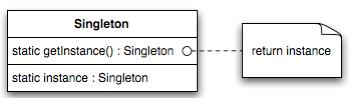
\includegraphics[width=0.5\linewidth]{images/singleton}
	\caption{Singleton}
	\label{fig:singleton}
\end{figure}


\subsubsection{Vorgehen}
\begin{enumerate}
	\item \lstinline|private| Default Constructor
	\item \lstinline|static getInstance()| Methode, welche die interne Instanz zurückliefert.
	\item \lstinline|static| Instanzvariable vom Typ der Singleton Klasse
\end{enumerate}

\subsubsection{Implementierung}
\begin{lstlisting}
public class Singleton {
	private volatile static Singleton uniqueInstance;
	
	private Singleton() {}
	
	public static Singleton getInstance() {
		if (uniqueInstance == null) {
		
			synchronized (Singleton.class) {
				// check twice. could be set in the meantime
				if (uniqueInstance == null) {
					// allocate space only if needed
					uniqueInstance = new Singleton();
				}
			}
		}
		
		return uniqueInstance;
	}
}
\end{lstlisting}

\clearpage


\subsection{Adapter}
\label{sec:adapter}
Das Adapter Pattern konvertiert die Schnittstelle einer Klasse in die Schnittstelle, die der Client erwartet. Adapter ermöglichen die Zusammenarbeit von Klassen, die ohne nicht zusammenarbeiten könnten, weil sie \textbf{inkompatible Schnittstellen} haben.
\begin{itemize}
	\item  Der Adapter ändert die Schnittstelle von einer existierende Klasse, damit sie dem Client entspricht.
	\item Der Adapter \textbf{kapselt} eine Klasse.
\end{itemize}

\subsubsection{Anwendungsfälle}
\begin{itemize}
	\item Das Entwurfsmuster findet in erster Linie Anwendung, wenn eine existierende Klasse verwendet werden soll, deren Funktion nicht ganz der geforderten enspricht.
\end{itemize}

\subsubsection{Varianten} 
Es gibt zwei Varianten von Adaptern:
\begin{description}
	\item[Objektadapter]: Verwendet Komposition
	\item[Klassenadapter]: Verwendet Mehrfachvererbung
\end{description}


\clearpage

\subsubsection{Objektadapter}
\begin{itemize}
	\item Auch als Wrapper bekannt
	\item Verwendet Komposition, welche zur Laufzeit hinzugefügt wird. Die Adapter Klasse besitzt also eine Instanzvariable vom Typ des Adaptee
	\item \textbf{Kapselt besser}, da die Methoden des Adaptee nicht sichtbar sind
	\item Alle Methoden die der Adapter zur Verfügung soll, müssen im Target Interface implementiert sein.
	\item Wird verwendet wenn man dem Client nur Methoden mit abgeänderter Adaptee Funktionalität zur Verfügung stellen möchte. Die restliche Adaptee Funktionalität soll aber versteckt bleiben.
\end{itemize}

\begin{figure}[h]
	\centering
	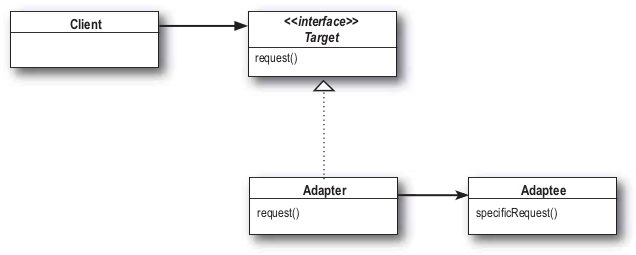
\includegraphics[width=0.7\linewidth]{images/adapter_pattern}
	\caption{Objektadapter}
	\label{fig:adapterpattern}
\end{figure}

\paragraph{Implementierung}
Der Objektadapter wird wie folgt verwendet
\begin{lstlisting}
public class Adapter implements Target {
	private Adaptee adaptee;
	
	public void request() {
		// convert, setup, etc.
		adaptee.specificRequest();
	}
}

public class Client {
	// Adapter hat eine Instanzvariable des Adaptee
	private Target myAdapter = new Adapter();
	
	public Client() {
		myAdapter.request();
	}
}
\end{lstlisting}


\clearpage

\subsubsection{Klassenadapter}
\begin{itemize}
	\item Verwendet Mehrfachvererbung welche bereits zur Compilezeit fixiert ist. Unter Java muss ein Interface und einer abstrakte Klasse verwendet werden, da Java keine Mehrfachvererbung unterstützt.
	\item Trägt die Methoden des Adaptees nach aussen
	\item Wird verwendet wenn eine zusätzliche Methode implementiert werden soll und man aber immer noch auf die  Methoden des Adaptee zugreifen soll.
\end{itemize}

\begin{figure}[h]
	\centering
	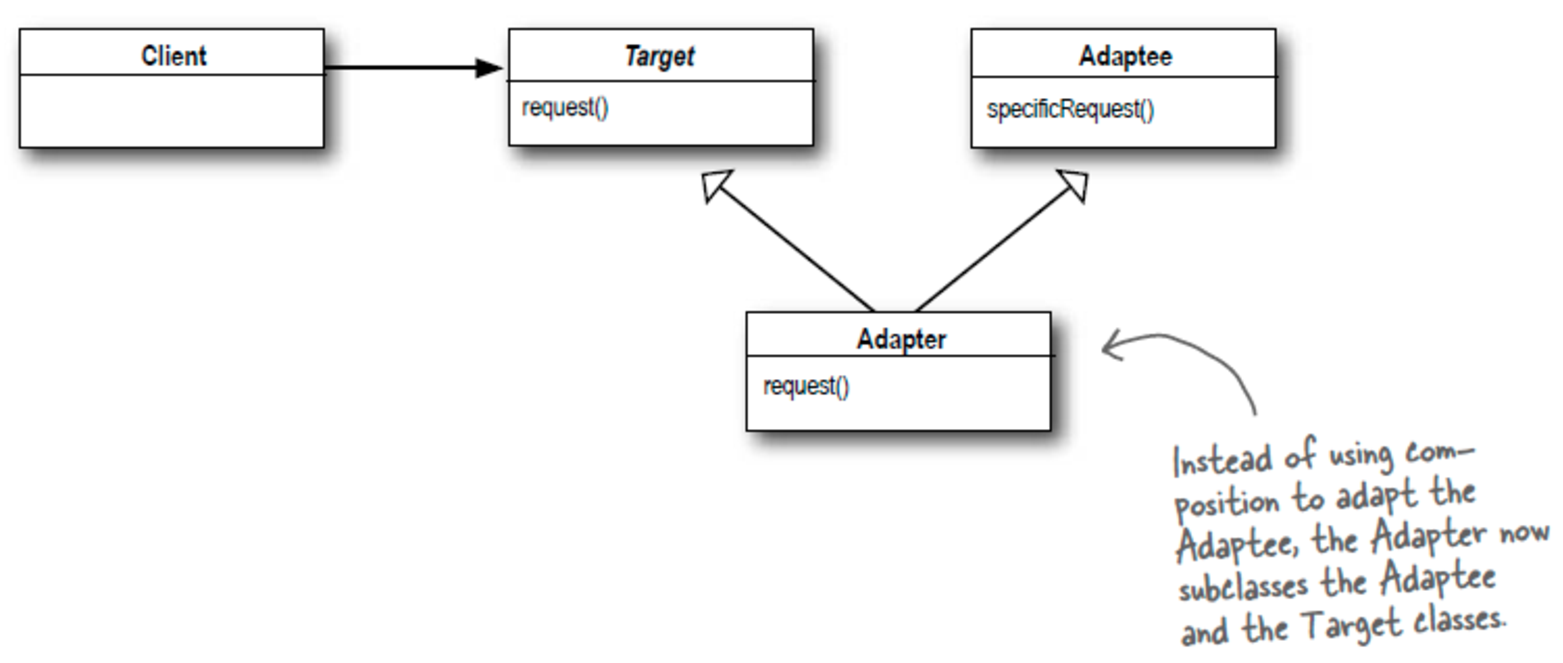
\includegraphics[width=0.7\linewidth]{images/adapter_class_pattern}
	\caption{Objektadapter}
	\label{fig:adapterpattern}
\end{figure}

\paragraph{Implementierung}
Der Klassenadapter wird wie folgt verwendet: 
\begin{lstlisting}
public class Adapter extends Adaptee implements Target {
	public void request() {
		super.specificRequest();
	}
}


public class Client {
	private Target myAdapter = new Adapter();
	
	public Client() {
		myAdapter.request();
		// Alle Adaptee Methoden sind wegen der Vererbung ebenfalls sichtbar
		myAdapter.anotherAdapteeMethod();
	}
}
\end{lstlisting}

\clearpage

\subsection{Facade}
\label{sec:facade}
Das Facade Pattern biete eine \textbf{vereinheitlichte Schnittstelle für einen Satz von Schnitstellen} eines Basissystems. Die Facade definiert eine hochstufigere Schnittstelle, die die Verwendung des Basissystems vereinfacht. 

\begin{itemize}
	\item Die Facade \textbf{vereinfacht die Schnittstelle} einer Gruppe von Klassen. 
	\item Die Facade abstrahiert die komplexe Verwendung mehrere Klassen für den Client weg.
	\item Die Facade kann im Gegensatz zum Adapter viele Klassen representieren
	\item Das Facade Pattern ist ähnlich wie der Adapter. Die Facade sollte immer dann verwendet werden, wenn eine grosse oder komplexe Schnittstelle vereinfacht werden muss. Der Adapter wird verwendet, wenn die gegebene Schnittstelle nicht der geforderten entspricht.
	\item Eine Facade entkoppelt einen Client von einem komplexeren Basissystem.
\end{itemize}

\begin{figure}[h]
	\centering
	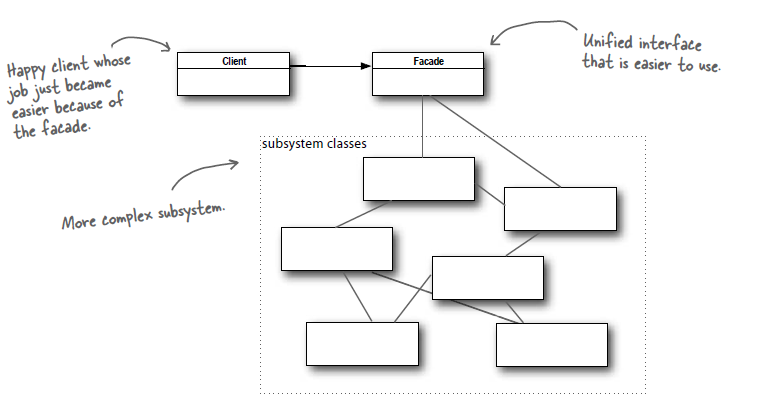
\includegraphics[width=0.9\linewidth]{images/fascade_pattern}
	\caption{Fascade}
	\label{fig:fascadepattern}
\end{figure}

\clearpage

\subsubsection{Implementierung}
\begin{lstlisting}
// Client
Facade facade = new Facade();
facade.doAction();

// Facade
public class Facade {
	private ISystem SystemComponentA a;
	private ISystem SystemComponentB b;
	private ISystem SystemComponentC c;
	
	public Facade() {
		a = new SystemComponentA();
		b = new SystemComponentB();
		C = new SystemComponentC();
	}
	
	public void doAction(){
		a.doAction();
		b.doAction();
		c.doAction();
	}
}


// 'Compelex' system
public interface ISystem {
	void doAction();
}

public class SystemComponentA implements ISystem {
	@Override
	public void doAction() {
		System.out.println("System Component A created");
	}
}

public class SystemComponentB implements ISystem {
	@Override
	public void doAction() {
		System.out.println("System Component B created");
	}
}

public class SystemComponentC implements ISystem {
	@Override
	public void doAction() {
		System.out.println("System Component C created");
	}
}
\end{lstlisting}


\clearpage

\subsection{Use Case Controller}
\label{sec:usecasecontroller}

\begin{itemize}
	\item Der Use Case Controller representiert ein oder mehrere Use Cases. 
	\item Der Use Case Controller bietet alle nötigen Operationen und Status Informationen um einen Workflow abzubilden.
	\item Die Daten hinter dem Use Case Controller können nur über ihn geändert werden
	\item Es können mehre Use Case Controller für einen Use Case existieren.
\end{itemize}

\subsubsection{Anwendungsfälle}
\begin{itemize}
	\item Wird klassisch in einem MVC Umfeld eingesetzt, wobei er mit einer Model Facade kommuniziert.
\end{itemize}

\begin{figure}[h]
	\centering
	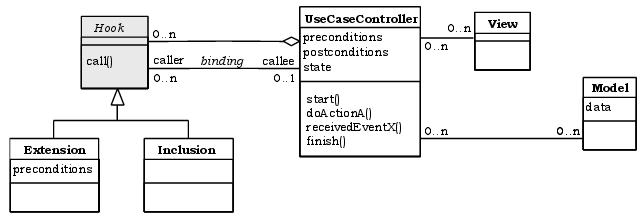
\includegraphics[width=0.7\linewidth]{images/usecasecontrolller_pattern}
	\caption{Use Case Controller}
	\label{fig:usecasecontrolllerpattern}
\end{figure}


\begin{lstlisting}
public class PlaceOrderUseCase extends UseCaseController {
	public void start() { .. }
	public void finish() { .. }
	public void displayForm() { .. }
	public void newItem() { .. }
	public void saveItem() { .. }
	public void submitOrder() { .. }
	public void cancelOrder() { .. }
}
\end{lstlisting}


\clearpage

\subsection{Composite}
\label{sec:composite}
Das Composite Pattern ermöglicht es, Objekte zu einer \textbf{Baumstruktur} zusammenzusetzen, um \textbf{Teil/Ganzes} Hierarchien auszudrücken. Das Composite Pattern erlaubt den Clients, individuelle Objekte und Zusammensetzungen von Objekten auf gleiche Weise zu behandeln.
\begin{itemize}
	\item Ein Composit enthält mehrere Komponenten, Diese sind entweder Composites oder Blatt Knoten.
	\item Eine Komponente ist eine Abstrakte Klasse, damit eine default Implementierung erstellt werden kann (seit neueren Java Versionen auch mit den Interfaces möglich)
	\item Die Leaf Knoten überschreiben nur diese Operationen die Sinn ergeben. Bei allen anderen Operationen wird die Default Implementierung verwendet.
	\item Die Composite Knoten überschreiben die Default Implementierung der abstrakten Klasse.
	\item Die Composite Knoten können selber nichts ausgeben. Sie delegieren die Operation nur an die Leafs.
	\item Die Default Implementierungen müssen nicht zwingend eine Exception werfen, sondern können auch sinnvollen Code enthalten.
	\item Bei teuren Durchquerungen des Trees, macht es evtl. Sinn die Zwischenergebnisse zu cachen.
	\item Der grösste Vorteil des Composit Pattern ist es, das ein Methodenaufruf einmalig getriggert und in der vollständigen Struktur aufgerufen wird. \item Clients behandeln Sammlungen von Objekten und einzelne Objekte auf die gleiche Weise
\end{itemize}

\begin{figure}[h]
	\centering
	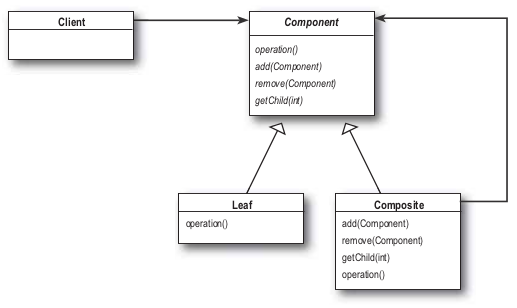
\includegraphics[width=0.6\linewidth]{images/composite_pattern}
	\caption{Composite}
	\label{fig:compositepattern}
\end{figure}

\subsubsection{Anwendungsfälle} 
\begin{itemize}
	\item GUI: Ein GUI besteht aus vielen Teilen. Bei der Anzeige, wird es jedoch als Ganzes betrachet. Man sagt der Top Komponenten, dass es sichtbar sein soll und dieses delegiert es an all seine Subkomponenten.
\end{itemize}



\subsubsection{Implementierung}
\begin{lstlisting}
public abstract class Component {
	public void add(Component c) {
		throw new UnsupportedOperationException();
	}
	
	public void remove(Component c) {
		throw new UnsupportedOperationException();
	}
	
	public Component getChild(int i) {
		throw new UnsupportedOperationException();
	}
	
	public String operation() {
		throw new UnsupportedOperationException();
	}	
	
	public void print() {
		throw new UnsupportedOperationException();
	}
}

public class Leaf extends Component {
	String name;
	
	public Leaf(String name) {
		this.name = name;
	}
	
	@Override
	public String operation() {
		return name;
	}
	
	@Override
	public void print() {
		System.out.println(getName());
	}
}

public class Composite extends Component {
	private List<Componet> componets = new ArrayList<>();
	private name;

	public Composite(String name) {
		this.name = name;
	}

	public void add(Component c) {
		componets.add(c);
	}
	
	public void remove(Component c) {
		components.remove(c);
	}
	
	public Component getChild(int i) {
		return (Component) components.get(i);
	}
	
	public String operation() {
		return name;
	}	
	
	public void print() {
		Iterator it = components.iterator();
		while(it.hasNext()) {
			Component c = it.next();
			component.print();
		}
 	}
	
}

// Client
// Creation could be done with a factoy
Component group = new Composite("all");

Component part1 = new Composite("part1");
Component part2 = new Composite("part2");

group.add(part1);
group.add(part2);

Component sub1 = new Leaf("sub1");
Component sub2 = new Leaf("sub2");

part1.add(sub1);
part2.add(sub2);

// prints all components
group.print();
\end{lstlisting}


\clearpage

\subsection{Decorator}
\label{sec:decorator}
Ein Decorator Muster fügt einem Objekt \textbf{dynamisch zusätzliche Verantwortlichkeiten} hinzu. Dekorierer bieten eine \textbf{flexible Alternative zur Ableitung} von Unterklassen zum Zweck der Erweiterung der Funktionalität.
\begin{itemize}
	\item Ein Decorator hat den gleichen Supertyp (Interface oder Abstrakte Klasse) wie die Objekte, die er dekoriert
	\item Komponenten können beliebig oft, dynamisch zur Laufzeit, dekoriert werden (verschachtelt)
	\item Jeder Decorator hat genau eine Instanzvariable, die eine \textbf{Referenz auf das Komponenten-Objekt} hält
	\item Decorator werden oft durch Factories oder Builder erstellt.
	\item Der Client muss nicht Wissen, dass er es mit einem Decorator zu tun hat.
\end{itemize}

\begin{figure}[h]
	\centering
	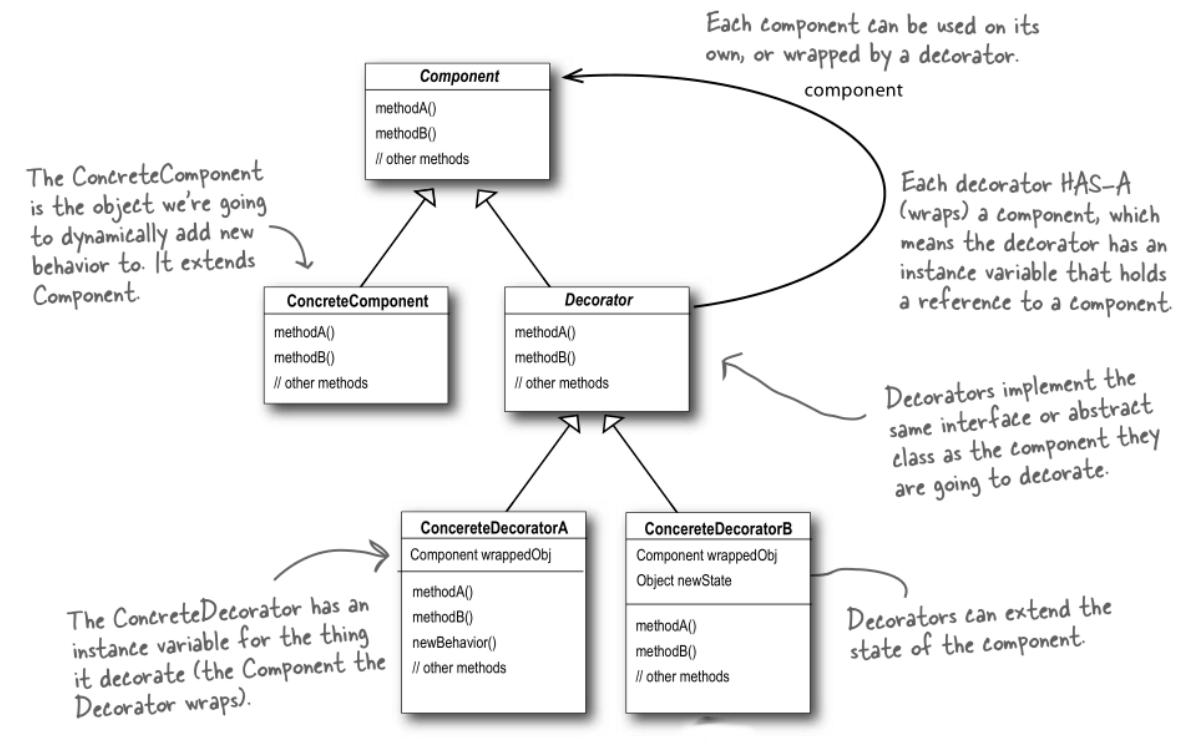
\includegraphics[width=0.7\linewidth]{images/decorator_pattern}
	\caption{Decorator}
	\label{fig:decoratorpattern}
\end{figure}

\subsubsection{Vorgehen}
\begin{enumerate}
	\item Gegeben ist eine Klasse \lstinline|Gertaenk| (Interface oder abstrakte Klasse)
	\item Erstelle eine Decorator Klasse (Interface oder abstrakte Klasse) und erbe von \lstinline|Gertaenk|
	\item Beliebige Subtypen von \lstinline|Gertaenk| erstellen
	\item Beliebig viele konkrete Klassen erstellen, die von Dekorator erben und eine Instanzvariable von \lstinline|Gertaenk| besitzen. Die Instanzvariable ist eine Referenz auf das eingepackte Objekt. (z.B Mit Zitrone, Mit Alkohol)
	\item Die einzelnen Objekte werden dem Konstruktor übergeben und so ineinander verschachtelt
\end{enumerate}

\subsubsection{Einschränkungen}
\begin{itemize}
	\item Decorator können nicht verwendet werden, wenn auf den Typ der konkrenten Komponenten geprüft werden muss.
	\item Ein Decorator kennt nie alle eingepackten Objekte, sondern nur das Nächste.
	\item Das Decorator Pattern verursacht viele kleine Klassen, weshalb man für die Erstellung der Decorator eine Factory Methode oder Builder nutzen sollte.
\end{itemize}

\subsubsection{Implementierung}
\begin{lstlisting}
// Abstract Component
public abstract class Component {
	
	public double getPrice() {
		// call abstract method
		return baseCost();
	}
	
	// abstract method
	protected abstract double baseCost();
}


// Multiple concrete Components
public class ConcreteComponent extends Component {
	@Override
	public double baseCost() {
		return 21;
	}
}


// Decorator extends Component
public abstract class Dekorationen extends Component {
	protected Component component;
}


// Concrete Decorator
public class ConcreteDecorator extends Decorator {

	// Wrap now inner component
	public ConcreteDecorator (Component component) {
		// pass to parent
		super.component = component;
	}
	
	@Override
	public double baseCost() {
		return component.basisKosten() + 4.5;
	}
}

// Client
Component c = new ConcreteComponent();
c = new ConcreteDecoratorA(c); // wrap component in decorator
c = new ConcreteDecoratorB(c); // wrap component in decorator
c.getPrice();
\end{lstlisting}

\clearpage

\subsection{Proxy}
\label{sec:proxy}
Das Proxy Pattern \textbf{kontrolliert den Zugriff} auf ein Objekt mit Hilfe eines vorgelagerten Stellvertreterobjekts.
\begin{itemize}
	\item Das Echte Subjekt und der Proxy implementieren die selbe Schnittstelle, damit den Stellvertreter am gleichen Ort wie das echte Objekt einsetzen kann.
	\item Der Proxy hält eine Referenz auf das echte Subjekt, dass die eigentliche Arbeit erledigt.
\end{itemize}

\subsubsection{Varianten}
Es gibt viele Proxy Varianten, wobei die drei wichtigsten die folgenden sind:
\begin{description}
	\item[Remote Proxy] Kontrolliert den Zugriff auf ein entferntes Objekt
	\item[Virtual Proxy] Kontrolliert den Zugriff auf eine Ressource, deren Erzeugung aufwändig ist
	\item[Protection Proxy] Kontrolliert den Zugriff auf eine Ressource mit genau festgelegten Zugriffsrechten
\end{description}

\begin{figure}[h]
	\centering
	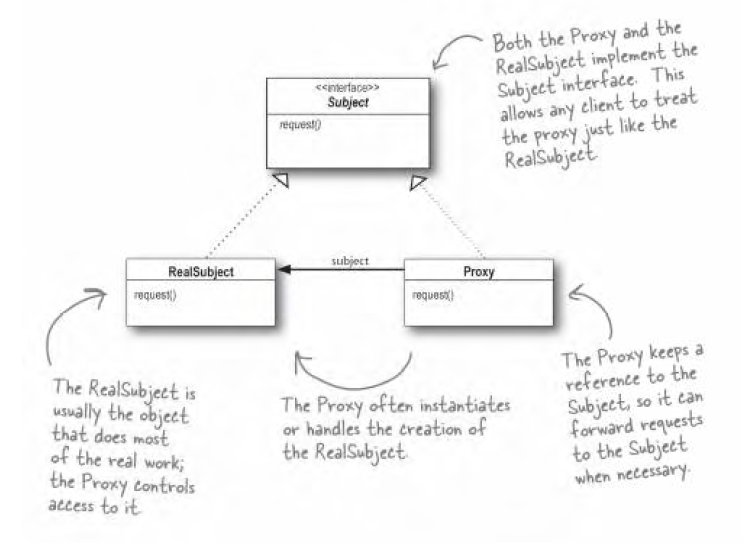
\includegraphics[width=0.9\linewidth]{images/proxy_pattern.png}
	\caption{Proxy}
	\label{fig:proxypattern}
\end{figure}

\clearpage

\subsubsection{Implementierung}
\begin{lstlisting}
// Subject
public interface Image {
	void display();
}

// Realsubject
public class RealImage implements Image {
	private String fileName;
	
	public RealImage(String fileName){
		this.fileName = fileName;
		loadFromDisk(fileName);
	}
	
	@Override
	public void display() {
		System.out.println("Displaying " + fileName);
	}
	
	// this gets called only once! (when realImage is null in proxy)
	// after that, image is loaded and can be displayed multiple times
	private void loadFromDisk(String fileName){
		System.out.println("Loading " + fileName);
	}
}

// Proxy
public class ProxyImage implements Image{
	private RealImage realImage;
	private String fileName;
	
	public ProxyImage(String fileName){
		this.fileName = fileName;
	}
	
	@Override
	public void display() {
		if(realImage == null){
			realImage = new RealImage(fileName);
		}
		realImage.display();
	}
}

// Client
Image image = new ProxyImage("test_10mb.jpg");
image.display(); 
\end{lstlisting}



\clearpage

\subsection{Command}
\label{sec:command}
Das Command Pattern kapselt einen Auftrag als ein Objekt und ermöglicht es so, andere Objekte mit verschiedenen Aufträgen zu paramatrisieren, Aufträge in \textbf{Warteschlangen} einzureihen oder zu protokollieren oder das \textbf{Rückgängigmachen} von Operationen zu unterstützen. Commands sind der \textbf{objektorientierte Ansatz von Callbacks}.
\begin{itemize}
	\item Kapsle die Aktion als Command Objekt und führe Sie zu einem beliebigen Zeitpunkt aus.
	\item Gibt allen Command Objekten eine gemeinsame Schnittstelle (oft \lstinline|execute()|)
	\item Statt \lstinline|action()| direkt aufzurufen, erzeuge das entsprechende Command Objekt, auf dem dann die Aktion ausgeführt wird.
	\item Es können mehrere Commands ausgeführt werden (Makro-Commands) 
	\item Commands können Rückgängig gemacht werden (besser Memento verwenden)
	\item Commands können gequeued und geloggt werden
	\item Oft wird der effektive Befehl im Receiver direkt im Command implementiert. Somit fällt der Receiver weg. Dieses vorgehen ist in der Praxis relativ gängig.
\end{itemize}

\subsubsection{Anwendungsfälle}
\begin{itemize}
	\item Transaktionssysteme (Während die Commands ausgeführt werden, werden sie auf gespeichert und können im Fehlerfall wiederhergestellt werden.)
\end{itemize}

\subsubsection{Vorgehen}
\begin{enumerate}
	\item Der Client ist verantworlich ein Command Objekt, ein Invoker und ein Receiver zu erstellen
	\item Der Client ruft \lstinline|setCommand()| auf, um den Command im Invoker zu speichern
	\item Später fodert der Client den Invoker auf, den Befehl auszuführen. 
	\item Der Invoker kann mehrer Commands als Instanzvariablen haben. Bei gegebenen Event werden alle diese Commands ausgeführt.
\end{enumerate}

\begin{figure}[h]
	\centering
	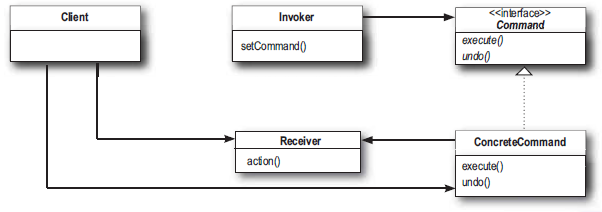
\includegraphics[width=0.7\linewidth]{images/command_pattern}
	\caption{Command}
	\label{fig:commandpattern}
\end{figure}

\subsubsection{Implementierung}
\begin{lstlisting}
public interface Command {
	public void execute();
	public void undo();
}

// Receiver
public class Light() {
	public void on() {
		// magic happens here
	}
}

// Concrete command
public class LightCommand implements Command {
	
	// Holds a receiver
	Light light;

	public LightCommand(Light light) {
		this.light = light;
	}
	
	public void execute() {
		// action might be directly implemented in command class
		light.on();
	}
	
	public void undo() {
		light.off();
	}
}

// Invoker
public class Remote() {
	// could also be single command
	private List<Command> commands = new ArrayList<Command>();
	private List<Command> undoCommands = new ArrayList<Command>();
		
	public void setCommand(Comman command) {
		this.commands.add(command);
	}
		
	// event
	public void buttonPressed() {
		for (Command command : commands) {
			command.execute();
			undoCommands.add(command);
		}
	}
	
	// undo event
	public void undoCommand() {
		for (Command undoCommand : undoCommands) {
			undoCommand.undo();
		}
		undoCommands.clear();
	}
}

// Client
Remote remote = new Remote(); // invoker
Light light = new Light(); // receiver
Command command = new LightCommand(light); // command
remote.setCommand(command);

remote.buttonPressed(); // trigger event
\end{lstlisting}

\clearpage



\subsection{Null Object}
\label{sec:nullobject}
\begin{itemize}
	\item Das Null Objekt wird immer dann verwendet, wenn man den Client davon befreien möchte, mit \lstinline|null| umzugehen. 
	\item Das Null Objekt ist eine \textbf{normale Klasse ohne Funktionilität}, die jedoch eine Schnittstelle implementiert.
	\item Das Null Objekt wird in vielen Pattern verwendet
\end{itemize}

\subsubsection{Implementation}
\begin{lstlisting}
// Null Objekt im Command Pattern
public class NullCommand implements Command {
	public void execute() { /* do nothing */ }
	public void undo() { /* do nothing */ }
}

// Null Object beim Iterator
public class NullIterator implements Iterator {
	public Object next() {
		return null;
	}
	
	public boolean hasNext() {
		return false;
	}
	
	public void remove() {
		throw new UnsupportedOperationException();
	}
}
\end{lstlisting}

\clearpage

\subsection{Observer}
\label{sec:observer}
Das Observer Pattern definiert eine \textbf{Eins-zu-viele-Abhängigkeit} zwischen Objekten in der Art, dass alle abhängingen Objekte benachrichtigt werden, wenn sich der Zustand eines Objekts ändert.
\begin{itemize}
	\item Das Subjekt hält die Daten und gibt Bescheid, wenn diese ändern. (Die Java Variante nennt das Subject Observable)
	\item Die Observer melden sich beim Subjekt an oder ab
	\item Beim Observer Pattern sind Subjekt und Observer locker gebunden. Das Subjekt arbeitet einzig mit dem Observer Interface.
	\item Bei der Java Variante kann man sich nicht auf die Reihenfolge der Benachrichtigung verlassen. Ebenfalls muss \lstinline|setChanged()| gesetzt werden.
	\item Der Observer ermöglicht es, eine Gruppe von Objekten zu benachrichtigen, wenn sich irgendein Zustand ändert.
\end{itemize}

\begin{figure}[h]
	\centering
	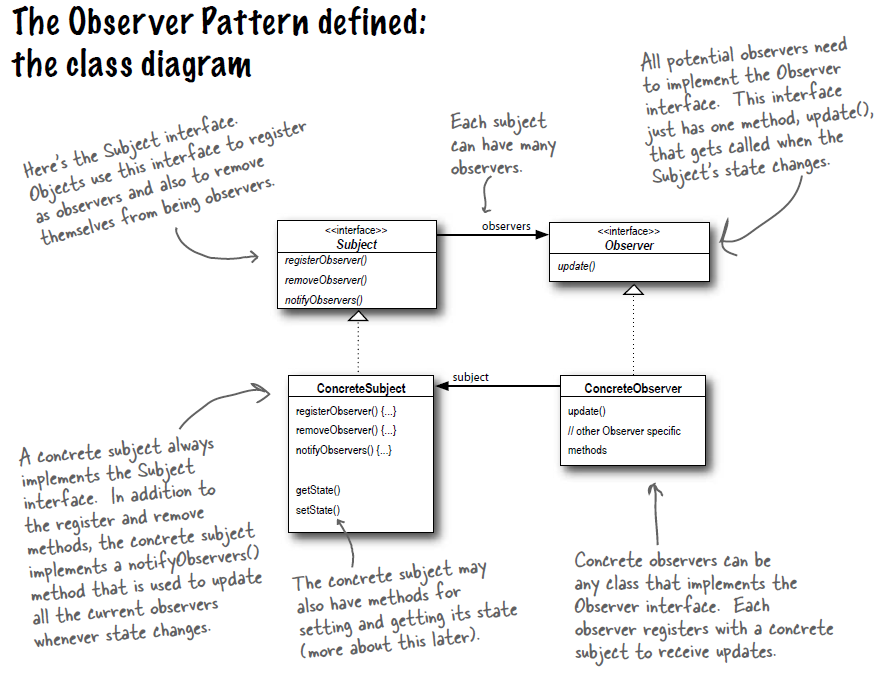
\includegraphics[width=0.65\linewidth]{images/observer_pattern}
	\caption{Observer}
	\label{fig:observerpattern}
\end{figure}

\subsubsection{Vorgehen}
\begin{enumerate}
	\item Erstelle ein Subjekt mit den Methoden \lstinline|register(Observer o)|, \lstinline|remove(Observer o)| und \lstinline|notify()|. Man erstellt immer ein Interface sowie ein konkretes Subjekt. Das konkrete Subject hält eine Liste von Observer, sowie die Werte die verteilt werden.
	\item Die Observer müssen das Interface \lstinline|Observer| implementieren. Das Observer Interface besitzt nur die Methode \lstinline|update(x,y,z)|, wobei die Parameter so gewählt sind, dass die Daten vom Subject übergeben werden können. Auch hier wird ein Interface und ein konkreter Observer erstellt. Jeder Observer registriert sich bei einem konkreten Subjekt.
\end{enumerate}

\clearpage

\subsubsection{Implementierung}
Ein Observer kann eigenhändigt erstellt werden oder man kann die vorhanden Klassen aus \lstinline|java.util| verwenden. Das konkrete Objekt würde in diesem Fall von \lstinline|java.util.Observable| erben und die konkreten Observer \lstinline|java.util.Observer| implmentieren. Damit die Observer benachrichtig werden muss zunächst die \lstinline|setChanged()| Methode augerufen und anschliessend einer der beiden Notify Methoden aufgerufen werden. (\lstinline|notifyObservers()| oder \lstinline|notifyObservers(Object arg)|). Beim konkreten Observer muss zusätzlich die Methode \lstinline|update(Observable o, Object arg)| überschrieben werden.
\begin{lstlisting}[caption=Eigener Observer]
// subject
public interface Subject {
	void registerObserver(Observer o);
	void removeObserver(Observer o);
	void notifyObservers();	
}

// Concrete Subject
public class MySubject implements Subject {
	private List<Observer> observers;
	private float myVal;
	
	public MySubject() {
		this.observers = new ArrayList<>();
	}
	
	public float getVal() {
		return myVal;
	}
	
	public void setVal(float newVal) {
		this.myVal = newVal;
		
		// value has changed, notify
		notifyObservers();
	}
	
	public void registerObserver(Observer o) {
		observers.add(o);
	}
	
	public void removeObserver(Observer o) {
		int i = observers.indexOf(o);
		if (i >= 0) {
			observers.remove(i);
		}	
	}
	
	public void notifyObservers() {
		for (Observer o : observers) {
			observer.update(myVal);
		}
	}
}





// Observer
public interface Observer {
	protected Subject subject;

	void update();
}

// Concrete Observer
public class MyObserver implements Observer {
	private float myVal;
	
	public MyObserver(Subject subject) {
		this.subject = subject;
		// register in subject
		this.subject.registerObserver(this);
	}

	public void update(float val) {
		// value in observable has changed
		this.myVal = val;
	}
}

// Client
Subject subject = new MySubject();

new MyObserverA(subject);
new MyObserverB(subject);
new MyObserverC(subject);

subject.setVal(55); // observers get notified

\end{lstlisting}
\clearpage

\subsection{State}
\label{sec:state}
Das State Pattern ermöglicht einem Objekt, sein Verhalten zu ändern, wenn sein interner Zustand sich ändert. Es scheint dann so, als hätte das Objekt seine Klasse gewechselt.
\begin{itemize}
	\item Mit dem State Pattern kann man zustandsabhängiges Verhalten umsetzen, ohne überall Fallunterscheidungen implementieren zu müssen
	\item Der Client kennt die Zustände oft nicht (nur der Context: Es ist Sache des Kontext seinen Zustand zu kontrollieren)
	\item Der Context delegiert sein Verhalten an die States, aus welchen er zusammengesetzt ist.
	\item Das State Pattern ist dem Strategy Pattern sehr ähnlich (\textbf{gleiches Klassendiagram, andere Absichten}), mit dem Unterschied, dass der Client kaum etwas über die States weiss und der Context die volle Kontrolle über das austauschen der States übernimmt. Beim Strategy Pattern sind die konkreten Instanzen hingegen meist fix programiert. (obschon es die Möglichkeit bietet, diese zur Laufzeit zu ändern)
\end{itemize}

\begin{figure}[h]
	\centering
	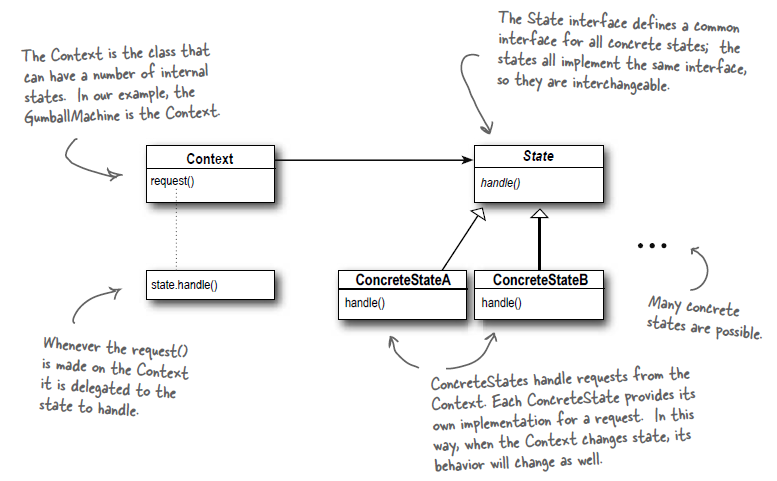
\includegraphics[width=0.65\linewidth]{images/state_pattern}
	\caption{State}
	\label{fig:statepattern}
\end{figure}

\subsubsection{Implementierung}
\begin{itemize}
	\item Sind die Zustandsübergänge \textbf{genau festgelegt}, ist die Logik dafür meist im Kontext abgelegt
	\item Sind die Zustandsübergänge \textbf{dynamischer}, ist die Logik meist in den Zuständen selber hinterlegt. (Mit dem Nachteil von Abhängikeiten zwischen den Zuständen)
\end{itemize}


\clearpage

\subsubsection{Vorgehen}
\begin{enumerate}
	\item Implementiere für jeden Zustand eine eignen Klasse
	\item Alle Zustandsklassen haben eine gemeinsame Schnittstelle
	\item Die Ausgangsklasse delegiert die zustandsabhängigen Methoden an diese Schnittstelle
	\item Jeder Zustandswechsel tauscht das aktuelle Zustandsobjekt aus
\end{enumerate}

\begin{lstlisting}
// state
public interface State {
	public void doAction(Context context);
}

// Concrete States
public class StartState implements State {
	public void doAction(Context context) {
		System.out.println("Start the game");
		context.setState(this);
	}
	public String toString() {
		return "Game is running";
	}
}

public class StopState implements State {
	public void doAction(Context context) {
		System.out.println("Stop the game");
		context.setState(this);
	}
	public String toString() {
		return "Game has stopped";
	}
}

// Context
public class Context {
	private State state;
	
	public Context() {
		state = null;
	}
	
	public void setState(State state) {
		this.state = state;
	}
	
	public State getState() {
		return state;
	}
}

// Client
Context context = new Context(); // context can change its state
State startState = new StartState();
startState.doAction(context);

State stopState = new StopState();
stopState.doAction(context);
\end{lstlisting}

\clearpage


\subsection{Strategy}
\label{sec:strategy}
Das Strategy Muster definiert eine Familie von Algorithmen, kapselt sie einzeln und macht sie austauschbar. Das Strategy Muster ermöglicht es, den Algorithmus unabhängig von Clients die ihn einsetzen, variieren zu lassen.
\begin{itemize}
	\item Das Strategy Pattern ist die flexible Alternative zur Vererbung
	\item Programmiere auf eine Schnittstelle und nicht auf eine Implementierung. Man nutzt dabei Polymorphismus, da der tatsächliche Objekttyp erst zur Laufzeit festgelegt wird.
	\item Identifiziere die Aspekte die sich ändern können und trenne sie von denen ab, die konstant bleiben.
	\item Komposition sollte der Vererbung vorgezogen werden, damit das Verhalten zur Laufzeit angepasst werden kann.
	\item Gelten viele Methoden in der Parent Klasse nur für einzelnene Child Klassen, sollte spezifisches Verhalten besser in Interfaces ausgelagert werden. Danach erstellt man mehrere Verhaltensklassen und zieht das Interface wieder in den Parent.
	\item Das Strategy Pattern ermöglicht einem Objekt, sein Verhalten zu ändern, wenn sich irgendein Zustand ändert
\end{itemize}

\begin{figure}[h]
	\centering
	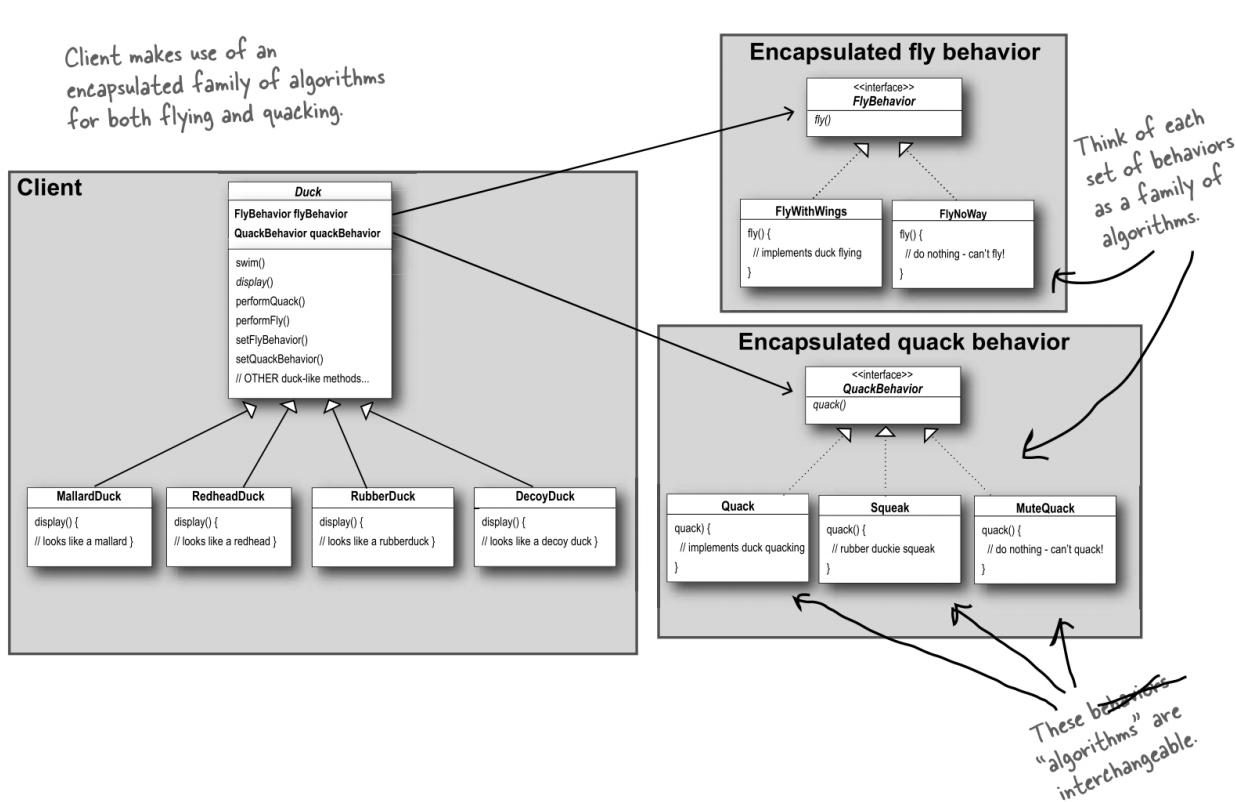
\includegraphics[width=\linewidth]{images/strategy_pattern}
	\caption{Strategy Pattern}
	\label{fig:strategypattern}
\end{figure}


\subsubsection{Implementierung}
\begin{lstlisting}
// Strategy
public interface Strategy {
	public int doOperation(int one, int another);
}

// Concrete strategies
public class OperationAdd implements Strategy {
	public int doOperation(int one, int another) {
		return one + another;
	}
}

public class OperationSubstract implements Strategy {
	public int doOperation(int one, int another) {
		return one - another;
	}
}

public class OperationMultiply implements Strategy {
	public int doOperation(int one, int another) {
		return one * another;
	}
}

// Client hold a behaviour (context)
public abstract class Calculator {
	private Strategy strategy;
	public Calculator(Strategy strategy) {
		this.strategy = strategy;
	}
	
	public int getResult(int num1, int num2) {
		return strategy.doOperation(one, another);
	}
}

public class Multiplier extends Calculator {
	public Multiplier() {
		super(new OperationMultiply());
	}
}

public class Adder extends Calculator {
	public Adder() {
		super(new OperationAdd());
	}
}

// Client
Calculator c1 = new Multiplier();
c1.getResult(2,3) // 6

c1 = new Adder();
c1.getResult(2,3); // 5
\end{lstlisting}


\clearpage

\subsection{Template Method}
\label{sec:templatemethod}
Das Template Method Pattern definiert in einer Methode das \textbf{Gerüst eines Algorithmus} und überlässt einige Schritte den Unterklassen. Template Method erlaubt Unterklassen, bestimmte Schritte des Algorithmus neu zu definieren, ohne die Struktur des Algorithmus zu ändern.
\begin{itemize}
	\item \textbf{Hook Methoden} sind Methoden, die in der abstrakten Klasse nicht tun oder nur ein Default Verhalten anbieten, aber in den Unterklassen überschrieben werden können.
	\item Um zu verhindern, dass Unterklassen den Algorithmus in der Template Methode ändern, wird die Template Methode als \lstinline|final| deklariert.
	\item Eine generelle Methode im Parent ruft dann alle Hoocks auf. Die gemeinsamen Teile werden in einer abstrakten Klasse implementiert und in den Subklassen bei Bedarf verfeinert.
	\item Die abstrakte Klasse besteht aus unveränderlichen Methoden welche zusätzlich abstrakte Methoden (Hooks) aufruft, welche in der Subklasse überschrieben werden müssen.
	\item Das Pattern verwendet das \textbf{Hollywood Prinzip}: Dont call us, we call you (Inversion of Control)
	\item Das Template Method Pattern erlaubt es viel Code wieder zu verwenden.
	\item Das Factory Method Pattern ist eine Spezialisierung des Template Method Pattern.
\end{itemize}

\subsubsection{Vorgehen}
\begin{enumerate}
	\item Definiere die Struktur des Algorithmus (Skelett) in der Basisklasse. Dieses Template Method ruft andere Methoden für die variierenden Details auf
	\item Diese anderen Methoden (Hook method)werden in den Unterklassen entsprechend überschrieben.
\end{enumerate}

\begin{figure}[h]
	\centering
	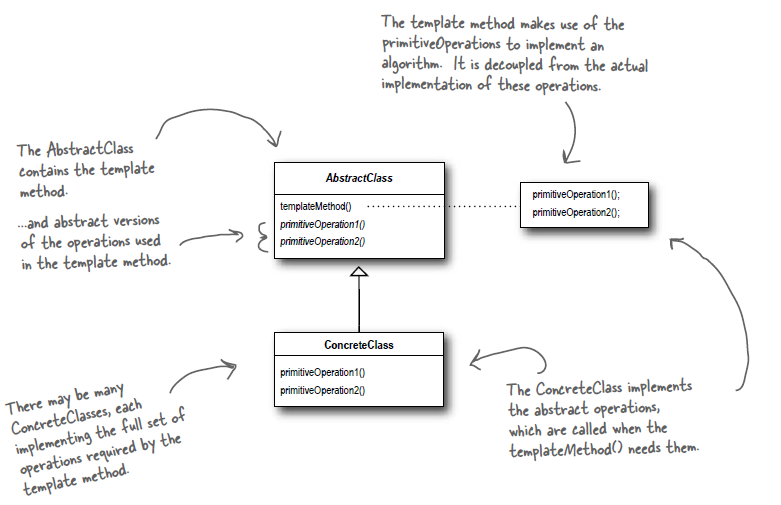
\includegraphics[width=0.7\linewidth]{images/template_method_pattern}
	\caption{Template Method}
	\label{fig:templatemethod}
\end{figure}

\subsubsection{Implementierung}
\begin{lstlisting}
public abstract class Game {
	// Hooks
	abstract void initialize();
	abstract void startPlay();
	abstract void endPlay();
	
	//template method
	public final void play(){
	
		//initialize the game
		initialize();
		
		//start game
		startPlay();
		
		//end game
		endPlay();
	}
}

public class Football extends Game {
	@Override
	void endPlay() {
		System.out.println("Football Game Finished!");
	}

	@Override
	void initialize() {
		System.out.println("Football Game Initialized! Start playing.");
	}

	@Override
	void startPlay() {
	System.out.println("Football Game Started. Enjoy the game!");
	}
}
\end{lstlisting}



\clearpage


\subsection{Iterator}
\label{sec:iterator}
Das Iterator Pattern bietet eine Möglichkeit, auf die Elemente in einem Aggregat-Object (Container) sequenziell zuzugreifen, ohne die zu Grunde liegende Implementierung zu offenbaren.
\begin{itemize}
	\item Iteratoren sind niemals sortiert, da die zugrundeliegende Struktur ein \lstinline|Set<T>| sein könnte. 
	\item Der Iteraotor bietet eine Möglichkeit, eine Sammlung von Objekten zu durchqueren, ohne die Implementierung der Sammlung zu offenbaren.
\end{itemize}

\subsubsection{Variaten}
Man unterscheidet zwischen externen und internen Iteratoren. 
\begin{description}
	\item[Externer Iterator] Ein externer Iterator wird vom Client mit \lstinline|next()| gesteuert, und erlaubt somit einen viel grösseren Grad an Flexibilität.
	\item[Interner Iterator] Ein interner Iterator wird vom Iterator selbst gestuert und ist somit weniger flexibler, dafür einfacher zu gebrauchen
\end{description}

\begin{figure}[h]
	\centering
	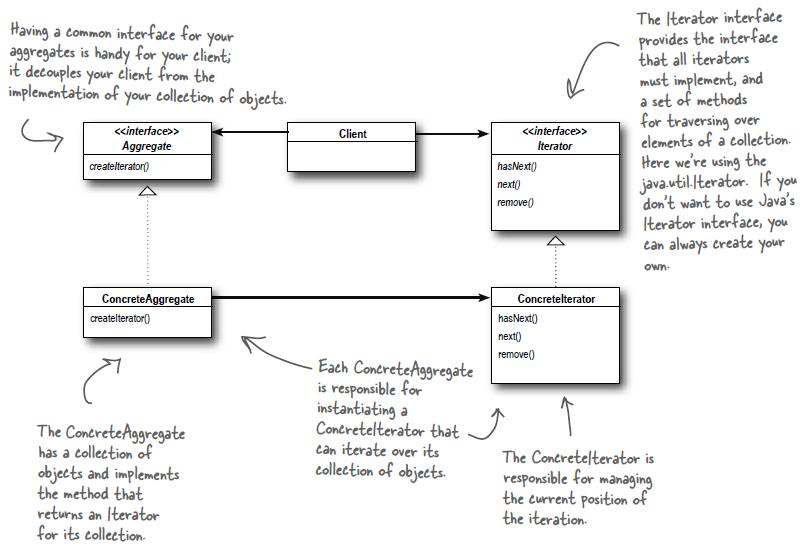
\includegraphics[width=0.9\linewidth]{images/iterator_pattern}
	\caption{Iterator}
	\label{fig:iteratorpattern}
\end{figure}

\clearpage

\subsubsection{Implementierung}
\begin{lstlisting}[caption=Iterator]
// Iterator
public interface Iterator {
	public boolean hasNext();
	public Object next();
}

// Aggregate
public interface Container {
	public Iterator getIterator();
}

public class NameRepository implements Container {
	public String names[] = {"Joe", "Lue", "Dave"};
	
	@Override
	public Iterator getIterator() {
		return new NameIterator();	
	}
	
	// Innerclass
	private class NameIterator implements Interator {
		int index;
		
		@Override
		public boolean hasNext() {
			if (index < names.length) {
				return true;
			}
			return false,
		}
		
		@Override
		public Object next() {
			if (this.hasNext()) {
				return names[index++];
			}
			return null;
		}
	
	}
	
}
\end{lstlisting}

\clearpage

\subsection{MVC: Model View Controler}
\label{sec:mvc}
Das MVC Pattern ist ein zusammengesetztes Muster, bestehend aus Observer, Strategy und Composite.
\begin{description}
	\item[Model] Die Daten und die Operationen auf den Daten. Es implementiert das Observer Pattern, um interessierte Objekte (Views, Controller) über Zustandsänderungen zu benachrichtigen
	\item[View] Darstellung der Daten. Implementiert das Composite Pattern. Wenn der Controller eine Aktualisierung der Views haben möchte, muss er es einfach der obersten View Komponenten sagen.
	\item[Controller] Nimmt Benutzereingaben entgegen und delegiert diese an das Model. Verwendete das Strategy Pattern damit die Controller in der View austauschbar sind.
\end{description}


\begin{figure}[h]
	\centering
	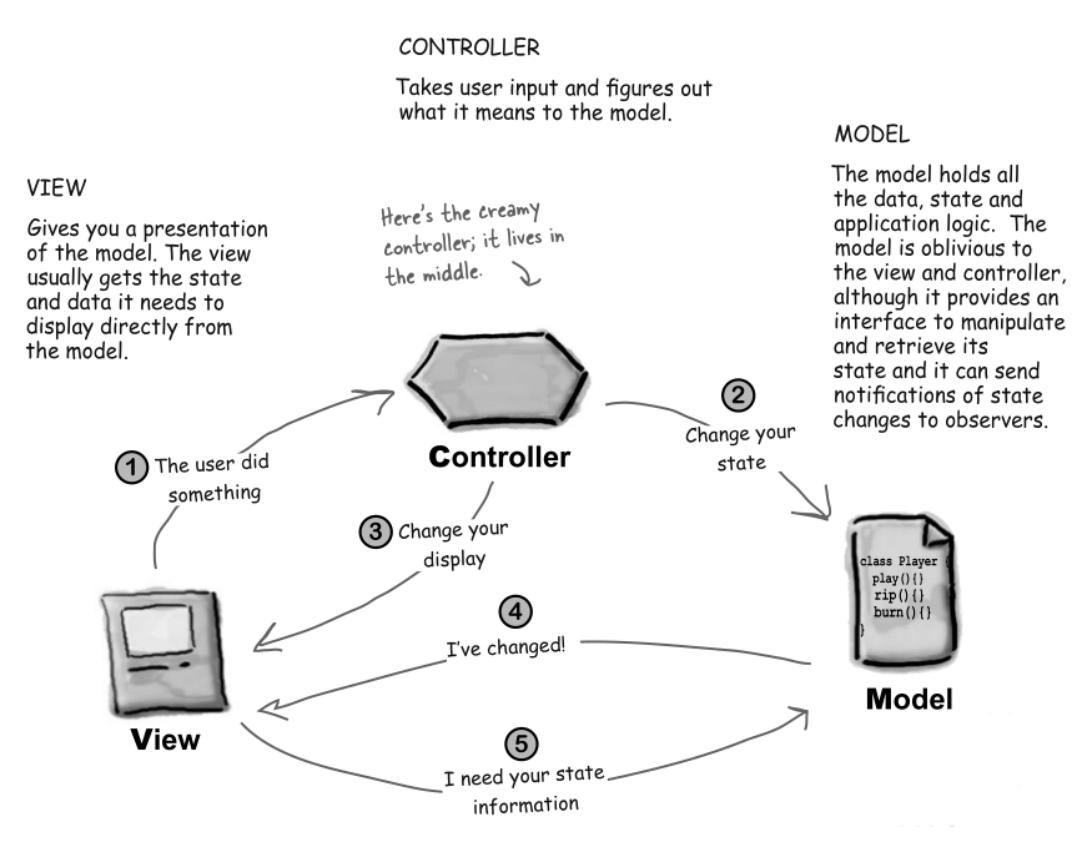
\includegraphics[width=0.7\linewidth]{images/mvc_pattern}
	\caption{MVC: Model View Controller}
	\label{fig:mvcpattern}
\end{figure}

\clearpage

\subsubsection{Implementierung}
\begin{lstlisting}
// Model
public class Student {
	private String rollNo;
	private String name;
	
	public String getRollNo() {
		return rollNo;
	}
	
	public void setRollNo(String rollNo) {
		this.rollNo = rollNo;
	}
	
	public String getName() {
		return name;
	}
	
	public void setName(String name) {
		this.name = name;
	}
}

// View
public class StudentView {
	public void printStudentDetails(String studentName, String studentRollNo){
		System.out.println("Student: ");
		System.out.println("Name: " + studentName);
		System.out.println("Roll No: " + studentRollNo);
	}
}

// Controller
public class StudentController {
	private Student model;
	private StudentView view;
	
	public StudentController(Student model, StudentView view){
		this.model = model;
		this.view = view;
	}
	
	public void setStudentName(String name){
		model.setName(name);		
	}
	
	public String getStudentName(){
		return model.getName();		
	}
	
	public void setStudentRollNo(String rollNo){
		model.setRollNo(rollNo);		
	}
	
	public String getStudentRollNo(){
		return model.getRollNo();		
	}
	
	public void updateView(){				
		view.printStudentDetails(model.getName(), model.getRollNo());
	}	
}

// Client
Student model = retriveStudentFromDatabase();
StudentView view = new StudentView();
StudentController controller = new StudentController(model, view);

controller.updateView();

//update model data
controller.setStudentName("John");
controller.updateView();
\end{lstlisting}

\section{GRASP}
Die \gls{grasp} Pattern beschreiben eine Menge von Entwurfsmuster, welche die Zuständigkeiten einer Klasse definieren. Die \gls{grasp} Pattern entstammen von Craig Larman.

\subsection{Information Expert}
Der Information Expert ist jene Klasse, welche die notwendigen Informationen besitzt, um eine Aufgabe zu erledigen. Eine Klasse muss alle Operationen bereitstellen, die mit ihr gemacht werden können. Diese Funktionsweise ist auch als \textbf{''Do it Myself''} Strategie oder \textbf{Kapselung} bekannt. Sie führt zu hoher Kohäsion und geringer Kopplung. 

\begin{itemize}
	\item Gutes Beispiel: Klasse \lstinline|Kreis|, mit dem Property \lstinline|radius| und der Methode \lstinline|berechneFlaeche()|
	\item Schlechtes Beispiel: Klasse \lstinline|BerechneFlaeche| mit einer Methode die eine geometrische Form entgegen nimmt.
\end{itemize}

\subsection{Creator}
Das Creator Prinzip legt fest, wer eine Instanz einer Klasse erstellt. Neue Objekte von der Klasse B sollten von A erzeugt werde, wenn:
\begin{itemize}
	\item A eine Aggregation von B ist (schwache Teil-Ganzes Beziehung)
	\item A, B-Instanzen enthält
	\item A, B-Objekte erfasst
	\item A, B-Objekte mit starker Kopplung
	 verwendet
	\item A die Initialisierungsdaten für B hat
\end{itemize}

\subsection{Controller}
Der Controller definiert, wer bestimmte Systemereignisse verarbeitet. Man unterscheidet zwischen Use-Case Controller und Facade Controller:
\begin{description}
	\item[Use Case Controller] Behandelt alle Ereignisse für einen Use Case
	\item[Facade Controller] Nimmt alle Meldungen entgegen und leitet sie an den richtigen Service weiter. (MessageHandler)
\end{description}

\subsection{High Cohesion}
Ziel von hoher Kohäsion ist es, den inneren Zusammenhalt einer Klasse hoch zu halten. Dass heisst, dass \textbf{eine Klasse für genau eine Aufgabe zuständig} ist.

\subsection{Low Coupling}
Ziel von geringer Kopplung ist es, so wenig Abhängigkeiten wie möglich, zu einer anderen Klasse zu haben. Dies erlaubt es, Anpassungen leichter durchzuführen, die Klassenfunktion leichter zu verstehen, einfacher zu testen und die Klasse besser Wiederverwenden zu könnnen. \\

Unter Kopplung versteht man folgende Dinge:
\begin{itemize}
	\item Vererbung
	\item Implementierung von Interfaces
	\item Halten von Instanzvariablen
	\item Benutzen von externen Methoden
\end{itemize}

\subsection{Polymorphismus}
Polymorphismus erlaubt es, das Verhalten abhängig vom Typ zu ändern. Somit können Fallunterscheidungen vermieden werden. (Siehe \ref{sec:strategy} Strategy Pattern)

\subsection{Pure Fabrication}
Eine Pure Fabrication Klasse (Reine Erfindung) gehört nicht zur Problem Domäne. Sie stellt oft Technologie Methoden zur Verfügung. Sie implemtentiert reines Verhalten und hat somit keinen Zustand.

\subsection{Indirection}
Indirection kann verwendet werden um geringe Kopplung zu erreichen. Bei der Indirection baut man einen Vermittler zwischen zwei Komponenten ein. (z.B Client / Server) Beispiel dafür ist der Controller, der zwischen Model und View vermittelt.

\subsection{Protected Variations}
Interfaces sollen immer verschiedene konkrete Implementierungen verstecken. Dadurch wird das System vor den Auswirkung eines Wechsels der Implementierung geschützt.

\section{Software Architektur}
Grosse Software Projekte werden in Schichten und Tiers unterteilt, damit Zuständigkeiten klarer werden, zusammengehörende Objekte gekapselt werden und Funktionalität explizit wiederverwendet wird. (Single Responsibility)

\subsection{Grundlegend}
\begin{itemize}
	\item Der Kunde ist oben der Service ist unten!
	\item Man greift immer von den oberen Schichten auf die Unteren zu. Das bedeutet dass die \textbf{unteren Schichten einen höheren Grad an Wiederverwendbarkeit} aufweisen. Die oberen Schichten sind von den unteren Abhängig.
	\item Oben ist man mehr Applikationsspezifischer
	\item Bei der Vererbung, sollte die Parent Klassen ebenfalls unten gezeichnet werden, da man somit konsistenter mit der Schichten Architektur (unten genereller) ist. Gleiches gilt für Klassendiagramme (n-Klasse oben bei 1:n Beziehung)
	\item In einem Klassen/Schichten Diagramm sollte nur die wichtigsten Klassen (meist das Interface gegen die oberen Schichten) gezeichnet werden
	\item Ein Architekturdiagramm nützt nur etwas wenn es kommunizierbar ist. Das Diagramm sollte deshalb maximal auf einem A3 Blatt platz finden.
	\item Die Namen der Schichten sind nicht standardisiert und können variieren.
	\item Verbreitet sind 3 und 6 Schichten Modelle.
\end{itemize}

\subsection{Motivation}
\begin{itemize}
	\item Schichten erlauben \textbf{bessere Wartbarkeit, Testbarkeit und Arbeitsaufteilung}
	\item Hat man saubere Schichten, können die einzelnen Schichten ohne weiteres ausgetauscht werden.
	\item Um eine hohe Kohäsion zu erreichen, sollten zusammengehörige Klassen in Packages gruppiert werden. Zusätzlich sollte eine Klasse nur für eine Aufgabe zuständig sein. (Single Responsibility)
\end{itemize}

\subsection{Einflüsse}
Die Architektur wird von verschiedenen Punkten beeinflusst. Den grössten Einfluss haben die \textbf{nicht-funktionalen Anforderungen}!
\begin{itemize}
	\item Deployment: Web? Mobile?
	\item Schwerpunkt: Analytisch? Grafik? Datenhaltung? Datentransfer? Game? 
	\item Performance
	\item Security
	\item Erweiterbarkeit
	\item Usability (enge Benutzerführung)
\end{itemize}


\subsection{Schichten}
Horizontale Schichten (''Wie der Code strukturiert ist''). Sie zeigen auf, wie die hierarchischen Abhängigkeiten sind. Die Aufrufe zwischen den Schichten sind synchron.
\begin{description}
	\item[UI] Zuoberst ist der \textbf{Presentation Layer}. Er zeigt die Daten an. (HTML, Reports, Windows)
	\item[Application Logic] Das GUI greift auf die \textbf{Use Case Controller} im Application Layer zu. Die Use Case Controller nehmen die GUI Anfragen entgegen und leiten sie an die unteren Schichten weiter. (Workflow)
	\item[DataAccess] Stellen funktionen für den Datenbank Zugriff zur Verfügung.
	\item[Business Domain] Hier sind die Services, welche die Request aus dem Application Layer verarbeiten.
	\item[Business Services] Beinhaltet Low Level Services für die Business Domain. Diese Klassen werden von mehreren Business Klassen verwendet. (z.B CurrencyConverter)
	\item[Libraries / Foundation] Zuunterst liegen die \textbf{Util Klassen} für Security, I/O, DB, Math Libraries, etc.
\end{description}

\begin{figure}[h]
	\centering
	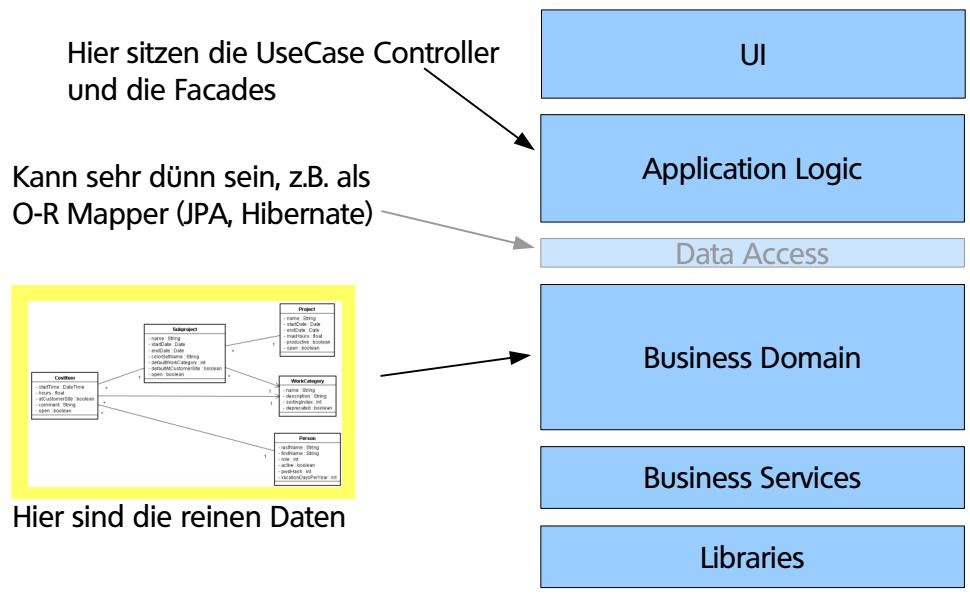
\includegraphics[width=0.7\linewidth]{images/architektur_layermodell}]
	\caption{Sechs-Schichten-Modell}
	\label{fig:architekturlayermodell}
\end{figure}


\begin{figure}[h]
\centering
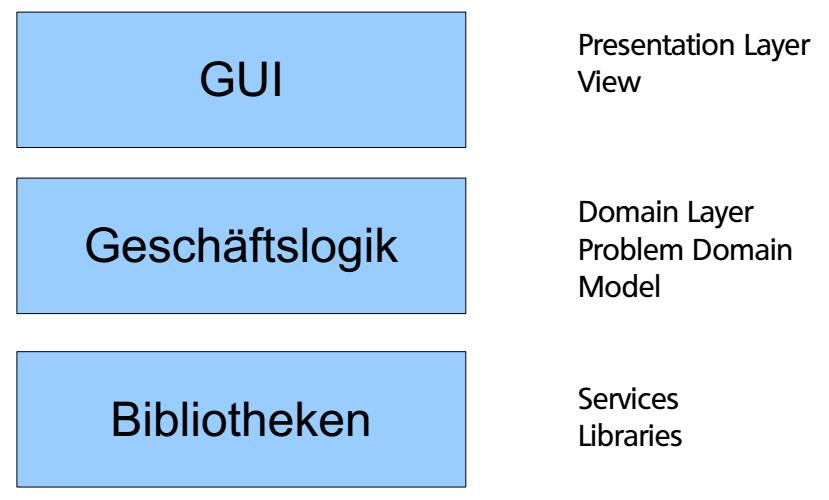
\includegraphics[width=0.35\linewidth]{images/three_tier_architecture}
\caption{Drei-Schichten-Modell}
\label{fig:threetierarchitecture}
\end{figure}

\subsubsection{Isolieren}
Gemeinsam verwendeter Code sollte in einer tieferen Schicht isoliert werden. Wird ein Code Fragment sehr oft aufgerufen, ist man unter Umständen gezwungen, die Aufrufe in die tiefere Schicht weiterzuleiten.
\begin{figure}[h!]
	\centering
	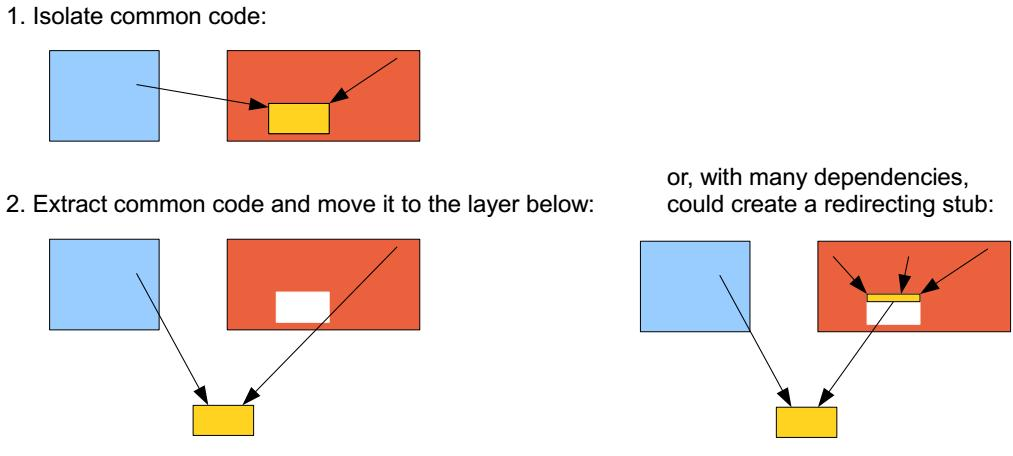
\includegraphics[width=0.7\linewidth]{images/layer_isolation}
	\caption{Isolierung von gemeinsamen Code}
	\label{fig:layerisolation}
\end{figure}

\subsubsection{Regeln}
\begin{enumerate}
	\item Aufrufe von oben auf die nächste darunterliegende Schicht sind immer OK
	\item Aufrufe nach unten, die eine Schicht überhüpfen sind manchmal auch OK
	\item Aufrufe innerhalb einer Schicht und Partition sind OK, sollten aber minimiert werden
	\item Aufrufe in einer Schicht quer zu einer anderen Partition sollten dringend vermieden werden
	\item Aufrufe NIE von unten nach oben, ausser callbacks (z.B. Observer pattern)
\end{enumerate}
\begin{figure}[h]
\centering
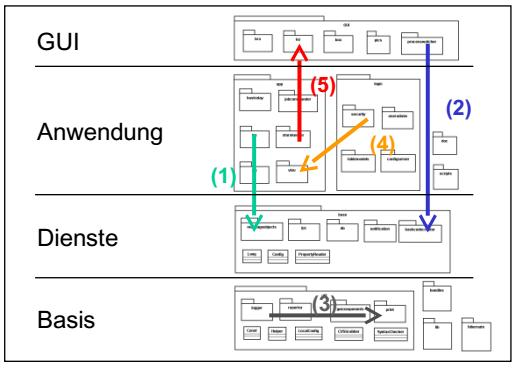
\includegraphics[width=0.6\linewidth]{images/dependency_rules}
\caption{Regeln für Abhängigkeiten}
\label{fig:dependencyrules}
\end{figure}

\subsection{Partitionen}
Eine Partition ist eine vertikale Unterteilung innerhalb einer Schicht. Die Kopplung zwischen den Partitionen sollte möglichst klein gehalten sein. Abhängigkeiten zwischen Klassen in zwei Partition derselben Schicht sollten vermieden werden. Falls die Abhängigkeit unumgänglich ist, sollte gemeinsamer Code isoliert werden und in eine tiefere Schicht verschoben werden. 

\subsection{Tiers}
Vertikale Ebenen von gleichberechtigten Laufzeitumgebungen (''Wo was läuft''). (User $\rightarrow$ Server $\rightarrow$ DB). Die Interfaces zwischen den Tiers sind asnychron. (d.h potentiell langsamer und somit teurer). In einem System werden n Schichten üblicherweise auf $n - x$ Tiers abgebildet (selten $n + x$). 


\subsection{Testing}
Das Unit Testing geht in der untersten Schicht am besten, da keine Abhängigkeiten bestehen. Je weiter hoch man geht, desto mehr Abhängigkeiten müssen weggemockt werden, um eine Schicht isoliert zu testen.


\subsection{Kohäsion und Kopplung}
Bei den Schichten  sollte eine hohe Kohäsion (Guter Zusammenhalt innerhalb der Klasse) und tiefen Kopplung(Minimierte Abhängigkeiten von andere Klassen) angestrebt werden. Mit einer tiefen Kopplung können die Komponenten einfacher ausgetauscht werden.
\begin{itemize}
	\item \textbf{Kopplung:} Wie stark ist eine Klasse Abhängig von vielen anderen Klassen. Aufrufe von einer Klasse zu anderen, von einem Package zum anderen
	\item \textbf{Kohäsion:} Zusammenhalt innerhalb einer Klasse. Ähnliche Dinge sollten in einer Klasse gruppiert werden. Kohäsion soll gegeben sein, sonst gehören die Dinge nicht ein eine Klasse/Package.
\end{itemize}

\begin{figure}[h]
	\centering
	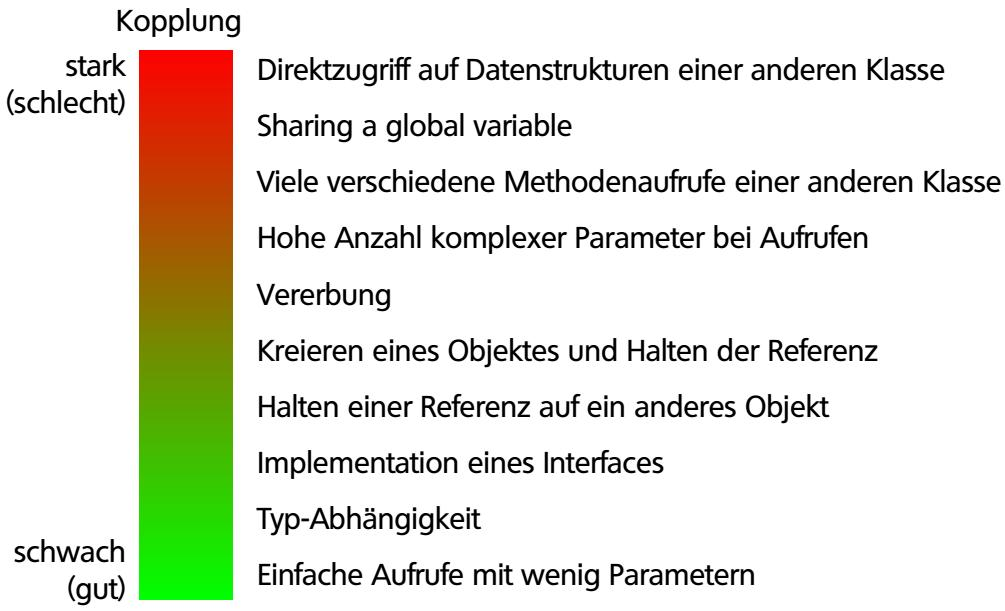
\includegraphics[width=0.7\linewidth]{images/kopplung_kohaesion}
	\caption{Arten von Kopplung}
	\label{fig:kopplungkohaesion}
\end{figure}


\section{Unified Process}
\begin{itemize}
	\item Beim veralteten Wasserfallmodell (Hermes) war das Problem, dass die Fehler von vorherigen Schritt mitgenommen wurden. 
	\item UP ist nur zu Beginn eine Art Wasserfall (aber auch da iterativ), nach End of Elaboration kann der Porzess voll agil sein.
	\item Der Unified Process ist für \textbf{kleinere und mittlere Projekte nicht geeignet}, da er 150 Aktivitäten, 40 Rollen und 80 Major Products definiert. 
	\item Analogie zum ''Weitersagen-Spiel''. Bei so vielen Rollen, kommt die Nachricht des Kunden vollkommen verzerrt beim Programmierer an. $p^{(n-1)}$ (p= angenommene Übertragungsqualität in Prozent)
	\item Jede Iteration hat ein lauffähiges Produkt zum Ziel. Immer ein Stück abliefern: Demo $\rightarrow$ Freude $\rightarrow$ wichtiges Feedback
	\item Der \textbf{wichtigste Meilenstein ist End of Elaboration}
	\item Die Arbeit kann erst über mehrere Teams aufgeteilt werden, wenn der Kunden verstanden wurde (Requirements, Keine Fragezeichen), die Architektur steht (Prototypen), UI steht (Wireframes, Prototypen), Zeitschätzung steht (Detailplanung), und die Tool Chain (IDE, Versionskontrolle, Build Server, Deployment, Unit Testing, Workflow Tools, Wiki) steht. (Zum Zeitpunkt End of Elaboration)
\end{itemize}

\subsection{Phasen}
Unified Processes werden in 4 Phasen eingeteilt. Die einzelnen Tätigkeiten können zwischen den Phasen fliessend übergehen und überlappen.
\begin{enumerate}
	\item \textbf{Inception}: Business Modelling, Requirements, Vision, Eckwerte (< 5\%)
	\item \textbf{Elaboration}: Analysis und Design (20-30\%). Ab diesem Punkt ist ein Abbruch noch relativ günstig möglich. 
	\begin{itemize}
		\item Technische Risiken beseitigt
		\item Prototyp erstellt
		\item Die Anforderung vollständig definiert (100\% Brief Use Cases und ca. 80\% fully dressed) 
		\item Detailierte Planung und Kostenschätzung
	\end{itemize}
	\item \textbf{Construction}: Implementation, Test, Deployment (viel Personal)
	\item \textbf{Transition}: Data Migration
\end{enumerate}

\begin{figure}[h!]
\centering
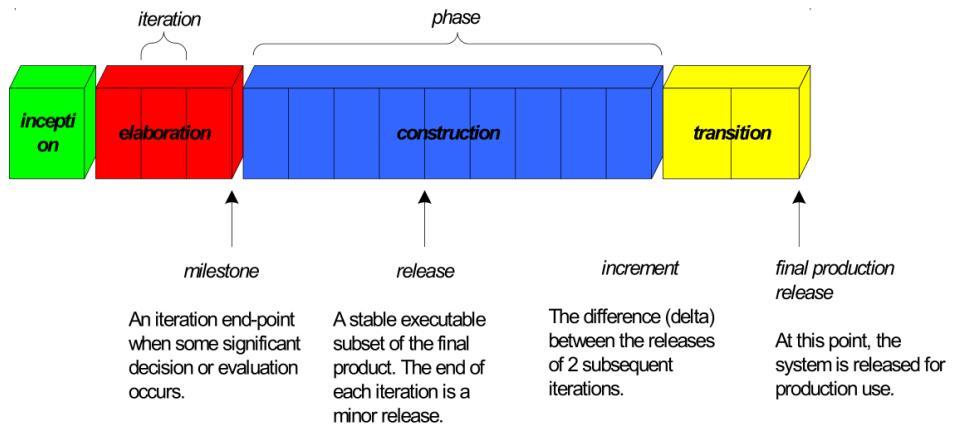
\includegraphics[width=0.9\linewidth]{images/unified_process}
\caption{Unified Process}
\label{fig:unifiedprocess}
\end{figure}

\section{SCRUM}
\begin{remember}{Goldene Regel}{}
	Enwickler schätzen, Kunde priorisiert
\end{remember}


\begin{figure}[h]
	\centering
	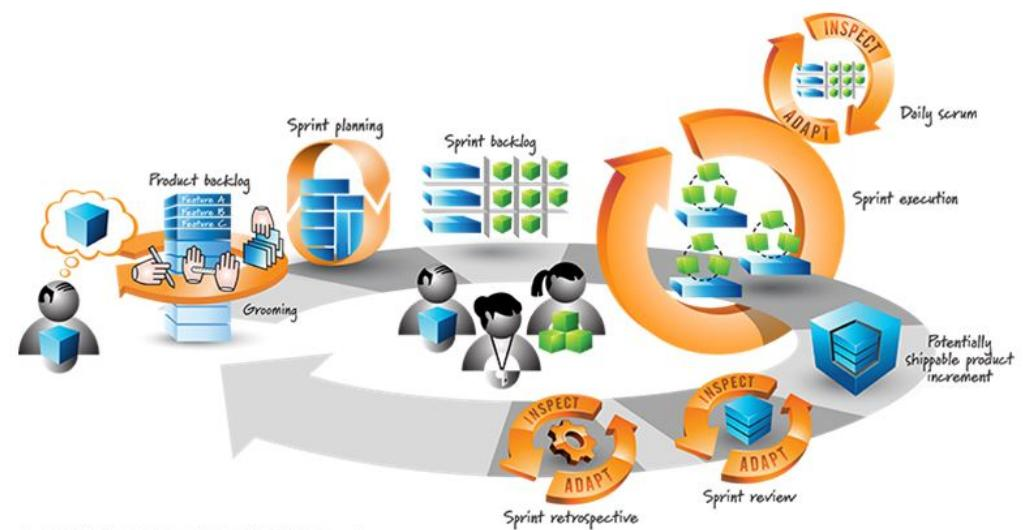
\includegraphics[width=0.9\linewidth]{images/scrum}
	\caption{SCRUM}
	\label{fig:scrum}
\end{figure}

\subsection{Terminologie}
\begin{description}
	\item[User Stories] \hfill \\
	Jede Story ist entweder Feature oder Bug. Eine User Story besteht aus vier Teilen:
	\begin{enumerate}
		\item Story Nummer
		\item Aufgabenbeschreibung: As a [user/role] I want to [goal] because [reason/motivation]
		\item Akzeptanzkriterien
		\item Aufwandschätzung (Story Points)
		\item Priorität
	\end{enumerate}
	\item[Epic]
	Epics sind Aufgaben auf Feature-Ebene, die viele User Storys umfassen.
	\item[Teamspeed/Velocity] \hfill \\
	Der Teamspeed passt sich von Iteration zu Iteration an. Er pendelt sich aber meist nach 3-4 Iterationen ein. Der Aufwand kann spielerisch mit Schätzpoker geschätzt werden.
	\item[Story Points] \hfill \\ 
	Story Points sind eine Einheit, die den Aufwand für das Umsetzen einer User Story beschreiben. Es geht dabei nicht nur um die Zeit sondern auch um die Komplexität.
	\newpage
	\item[Product Backlog] Nach Priorität sortierte Liste aus User Stories.
	\item[Backlog Board] \hfill \\
	Das Backlog Board ist in zwei Bereiche unterteilt. Die Story Area beinhaltet die User Stories und die Constraint Area die Vorgaben. Oft werden Post Its (Story Cards) in Gelb (Anforderung) und Rot (Bug) verwendet. 
	\begin{figure}[h!]
		\centering
		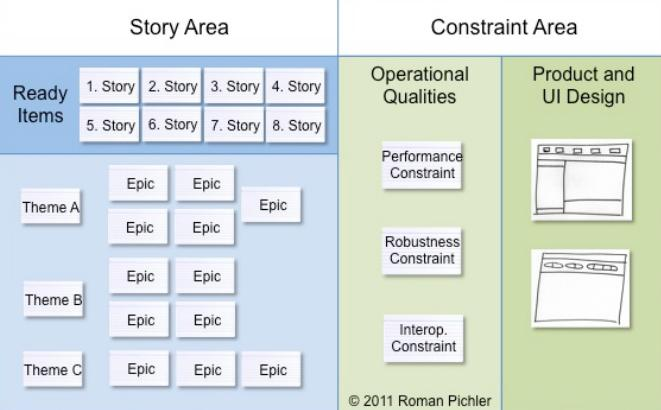
\includegraphics[width=0.5\linewidth]{images/productbacklog}
		\caption{Backlog Board}
		\label{fig:productbacklog}
	\end{figure}
	\item[Sprint] \hfill \\
	Sprints sind iterative Aufteilungen des Workloads in fixe Zeitintervalle. Ein Sprint dauert traditionell 2-3 Wochen. Alle Sprints dauern gleich lange. Das Intervall ist fix. Wird eine Story im Sprint nicht fertig, kommt es in den nächsten Sprint. (auch 98\% fertige Stories)
	\item[Sprint Backlog] \hfill \\
	So viel Arbeit wie das Team in einem Spring bewältigen kann, kommt in den Sprint Backlog. Pro Sprint wird nur das bearbeitet, was im Sprint Backlog liegt. (Niemals weitere Anforderungen aus dem Product Backlog).
	\item[Scrum Task Board] \hfill \\
	Das Task Board visualisiert den Status der einzelnen Subtasks einer User Story im Sprint Backlog. (TODO, In Process, To Verify, Done)
	\begin{figure}[h!]
		\centering
		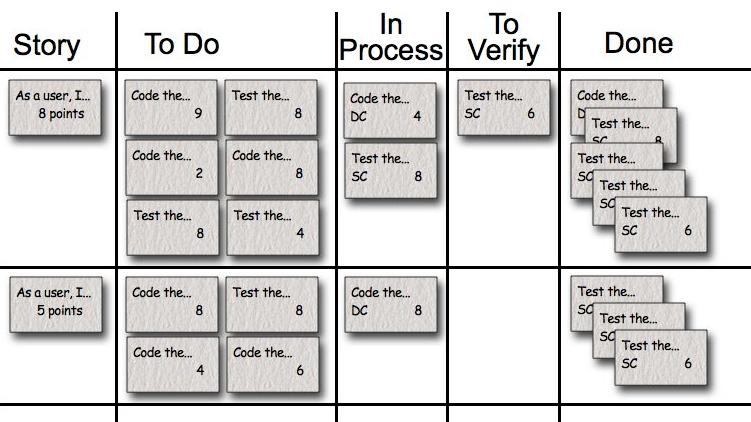
\includegraphics[width=0.6\linewidth]{images/scrum_task_board}
		\caption{SCRUM Task Board}
		\label{fig:scrumtaskboard}
	\end{figure}
\end{description}

\subsection{Ereignisse}
\begin{description}
	\item[Sprint Planning] \hfill \\
	Beim Sprint Planning wird so viel Arbeit, wie ein Team bewältigen kann in den Sprint Backlog verschoben. Dies geschieht immer am Anfang eines Sprints.
	\item[Daily Standup Meeting] Beim Daily Standup Meeting bekommt jeder Enwickler max. 2min Zeit. Es wird gesagt, an was man gerade arbeitet und wo eventuelle Probleme liegen. Es geht darum, zu wissen, was die anderen machen.
	\item[Sprint Review] \hfill \\
	Am Schluss jedes Sprint gibt es eine Demo für den Kunden/Product Owner. Der Product Owner nimmt alle Features ab und es gibt eine Diskusion, was wirklich abgeschlossen ist. Der neue Speed wird hier definiert. 
	\item[Sprint Retrospective]
	Regelmässig am Schluss eines Sprints gibt es ein kurzes Meeting, um das Erledigte zu reflektieren. Was ist gut gelaufen? Was hat Probleme bereitet? Was kann man verbessern?
\end{description}

\subsection{Rollen}
\begin{description}
	\item[Product Owner] Ist verantwortlich, dass das Richtige gemacht wird. Er ist oft Teil der Firma des Auftraggebers. Oft sind das Produktmanager der Firma. Er kennt das Business. Ideal ist es, wenn der Product Owner im gleichen Büro wie das Enwicklungs-Team ist und ständig ansprechbar ist.
	\item[Scrum Master] Es gibt einen SCRUM Master pro ca. 5 SCRUM Teams. Der SCRUM Master kennt sich sehr gut mit SCRUM aus und hilft bei allfälligen Schwierigekeiten.
	\item[Enwickler Team] Die Entwickler setzen die Aufgaben gemäss ihren Kenntnissen und Fähigkeiten um. (Programmieren, Testen, User Stories Schreiben, User Expreience, UI Design, Architektur und Design, Netzwerk und Server)
\end{description}

\clearpage

\subsection{Vorgehen}
\paragraph{Requirements Analysis}
\begin{enumerate}
	\item Product Backlog erstellen
	\item Backlog Grooming: Das Team und der Product Owner diskutieren zusammen, bis alle Anforderungen verstanden sind
	\item Das Team definiert die Kosten pro User Story (Story Points). Geht eine Story länger wie ein Sprint, muss sie aufgeteilt werden.
	\item Der Product Owner priorisiert den Product Backlog nach seinen Prioritäten
	\item Teamspeed definieren: Speed = Anz. fertig gestellter Story Points pro Sprint - Reserveren (Krankheit, Militär, Feiertage)
\end{enumerate}

\paragraph{Sprint Planen}
\begin{enumerate}
	\item Sprints einplanen: Der Kunde wünscht oft ein Datum, wann das Projekt abgeschlossen ist. Da SCRUM ein iterativer Prozess ist und das Kundenbudget nicht unendlich ist, ist dies schwierig zu definieren. Grundsätzlich kann man aber die geschätze Zeitdauer aller User Stories durch den Teamspeed teilen. 
	\item Die am höchsten priorisierten User Stories in den Sprint Backlog verschieben.
	\item Nach dem Sprint soll immer eine lauffähige Version zur Verfügung stehen.
	\item Stories die nach einem Sprint nicht abgenommen oder abgeschlossen sind, werden in den nächsten Sprint verschoben. Ebenfalls muss der Zeitaufwand neu geschätzt werden.
	\item Erledigte User Stories werden in den Product Backlog zurück verschoben und als erledigt markiert.
	\item Danach wird der nächste Sprint geplant. Die Prioritäten werden unter Umständen neu gesetzt und nicht abgeschlossene/abgenommene User Stories kommen in den neuen Sprint. Bei nicht abgeschlossenen User Stories muss der Zeitaufwand neu geschätzt werden. Ebenfalls wird der Aufwand dem neuen Teamspeed angepasst. Es ist dem Team auch frei, den Teamspeed selbständig hochzusetzen.
	\item Die vorgehenden Schritte werden nun iterativ wiederholt.
\end{enumerate}


\section{Projektmanagement}
\subsection{Anforderungen}
\paragraph{Die vier Projekt-Variablen} \hfill
\begin{enumerate}
	\item Kosten / Aufwand / Personen (einfach zu verstehen/messen)
	\item Zeit 
	\item Funktionalität (schwieriger zu verstehen/messen)
	\item Qualität (sehr schwierig zu verstehen/messen)
\end{enumerate}

\paragraph{Kunde verstehen} \hfill \\
Im Idealfall ist der Kunde im Team und bekommt die Änderungen direkt mit. Worte können missverstanden oder anders interpretiert werden. Hilfreich sind verständlich geschriebene Anforderungen, Use Cases, nicht funktionale Anforderungen oder Prototype und grafische Entwürfe. Es hilft auch, mit dem Team vor Ort den Businessprozess anzuschauen.

\paragraph{So früh wie möglich so formal wie möglich} \hfill \\
Je früher man formal wird, desto mehr Zeit spart man sich später. (UML, halb formale Text: Use Cases, Risikolisten, Tests). Bilder können Projekte retten.

\paragraph{Die hohe Kunst: Sichtbar machen} \hfill \\
Software ist für Nicht-Programmierer unsichtbar. Es gilt das unsichtbare, also den Fortschritt, die Ideen und Konzepte (Architektur, Design, Schnittstellen) mit Diagrammen (Domainmodell, Activitydiagramme, Statediagramme ,Contextdiagramme, Sequnezdiagramme, Package und Deployment Diagramme) sichtbar zu machen. Es gibt noch weitere Variaten um den Projektverlauf zu visualisieren:
\begin{itemize}
	\item Burn-down chart
	\item Bug count
	\item Time to fix bugs
	\item Build breaks
	\item Metriken (Klassenlänge, Verschachtlungen)
\end{itemize}

\subsection{Scope Keeper} \hfill \\
Der ProjektManager muss den Funktionsumfang des Projekts im Zaum halten. Dies ist der \textbf{wichtigste Punkt}! Wenn man dies nicht umsetzt, dann kann man noch so ein tolles Team haben, die sauberste Architektur entworfen haben, mit den besten Werkzeugen und Techniken arbeiten: Man kann das Projekt rauchen.
\begin{itemize}
	\item 2\% an unerwarteten Erweiterungen (Scope Creep) pro Monat sind normal. Folglich können 20 Monate lange Projekte um 40\% umfangreicher werden. 
	\item Plane kein Projekt über mehr als neun Monate. Ansonsten sollte es aufgeteilt und auch so verkauft werden.
\end{itemize}


\subsection{Communication is Key}
\paragraph{Software ist Kommunikations-intensiv} \hfill
\begin{itemize}
	\item Das Team sollte an einem Ort sein und die selbe Sprache sprechen
	\item Teamwand einrichten. (SCRUM Board)
	\item Viel und regelmässig austauschen (Daily Standup Meeting)	
\end{itemize}

\subsection{Kosten}
\paragraph{Entfernung ist teuer} \hfill \\
Im Idealfall arbeitet das ganze Team im selben Gebäude und Stockwerk. Ansonsten gibt es höhere Kosten
\begin{itemize}
	\item +10\%: Alle arbeiten im selben Gebäude, aber nicht mehr auf einem Stock
	\item +10\%: Alle arbeiten in derselben Ortschaft, aber nicht mehr im gleichen Gebäude
	\item +10\%: Alle arbeiten im gleichen Land, ...
	\item +10\%: Alle arbeiten in derselben Zeitzone
	\item +10\%: nicht mehr gleiche Zeitzone, Zeitverschiebung mehr als 4 Std.
	\item +20\%: Nicht alle haben dieselbe Muttersprache (= Kommunikationssprache)
\end{itemize}

\paragraph{Übergaben sind teuer} \hfill \\
Wenn man eine Arbeit jemand anders übergeben muss, dann kostet das einen erheblichen Aufwand und es ist mit Kommunikationsfehlern zu rechnen. Um diesem Problem entgegen zu wirken, kann man wichtigen Rollen auf zwei Personen aufteilen (Pilot/Copilot). Ebenfalls sollte der Software Architekt bereits früh im Projekt involviert sein. Auch hier begünstigt die örtliche Nähe den Informationsaustausch.

\subsection{Praktische Tipps}
\paragraph{Nichts vergessen dank Listen} \hfill
\begin{itemize}
	\item Tasks für das Entwicklungsteam in Ticketing Tool erfassen
	\item ToDo Liste führen über Dinge, die aus dem Weg geräumt werden müssen
	\item Maximal drei Prioritäten definieren (1. dringen, 2. wichtig, 3. machen wenn Zeit)
\end{itemize}

\paragraph{Immer iterativ  vorgehen} \hfill \\
Agile Methoden haben sich bewährt weil:
\begin{itemize}
	\item Kunde sieht immer wieder Resultate und kann Feedback geben
	\item Das Team hat Zwischenresultate, die ein Gefühl von “wir haben was geschafft!“ vermitteln.
	\item Es ist einfacher, ein System schrittweise auf- und auszubauen (mit Refactoring) als eine “Big Bang” Integration gegen Schluss zu machen.
	\item Fehler und Fehleinschätzungen („das will der Kunde so“) werden früher entdeckt.
	\item Auch Requirements iterativ erfassen (mit OOA zwischendrin)
	\item Sprints: 2-3 Wochen Dauer, Kunden-Demos: alle 2-3 Monate
\end{itemize}

\paragraph{Inspect - Adapt} \hfill \\
Ein Projekt sollte als eine Reise betrachtet werden. Unerwartete Erreignisse sollten erkannt und die Reise entsprechen angepasst werden. Das Gegenteil wäre ein abgeschossener Pfeil, dessen Richtung sich nicht mehr ändert. 


\paragraph{Projektkontrolle} \hfill
\begin{itemize}
	\item Budgetkontrolle
	\item Fortschrittskontrolle. Aktiv nachfragen und Probleme lösen. Es darf nicht vorkommen, dass ein Programmierer über Wochen am gleichen Problem arbeitet.
	\item Management by walking around: Anwensenheit schafft Verbindlichkeit
	\item Hotspots identifizieren: Hotspots sind Dinge, die niemand übernehmen möchten. Dinge, die immer wieder geändert werden müssen.
\end{itemize}

\paragraph{Gehen Sie auf die Baustelle} \hfill
\begin{itemize}
	\item Ein Projektleiter muss selbständig den aktuelle Stand der Baustelle (Versionierungstool) kennen.
	\item Commits im Versionierungstool überprüfen. Warum gibt es keine Commits? (Code anschauen, Diffs anschauen, Tests überprüfen)
	\item Welche Codeteile haben sich oft geändert?
	\item Welche Codeteile werden oft gebraucht?
\end{itemize}

\paragraph{Geschichtsbeschreibung} \hfill \\
Das erste Projekt wird wahrscheinlich schief laufen. Man sollte sich deshalb die wichtigsten Punkte (Lessons learned) notieren und eine Schlusspräsentation halten. (Export von Redmine, Screenshots von Milestones und Schwierigkeiten, Sitzungsprotokolle, Mitarbeiterzufriedenheit, Kundenzufriedenheit, Fehlerquellen)

 
\section{Redmine}
Redmine ist ein Open Source Projektmanagement Werkzeug wie JIRA. Es wird hauptsächlich für folgende Dinge verwendet:
\begin{itemize}
	\item Tasks erfassen (Features)
	\item Bug, Issue Tracking
	\item Versionskontrolle Integration (Git, SVN)
	\item Wiki (für Protokolle, How-To's, Milestone Reviews), User Forum, Dokumente, Files
	\item Release Planung
	\item Rollenbasierte Zugriffskontrolle für Benutzer
	\item Stundenerfassung
\end{itemize}

\appendix

% Code Listings
\lstlistoflistings

% List of figures
\listoffigures

% List of tables
\listoftables

% Bibliography
\bibliographystyle{plain} 
\bibliography{literatur}

\end{document}